\chapter{Zero-intervals}
\label{chap:ints}
In Chapter~\ref{chap:chars}, we characterized matrices avoiding small patterns. Their structure is very dependent on the pattern they avoid and the results are hard to generalize for arbitrary patterns. In this chapter, we look for a more general property that restricts the complexity of a class of matrices.

\begin{defn}
For a matrix~$M\in\Mat$, a row interval $M[\{r\},[c_1,c_2]]$ is a \emph{zero-interval} if all entries are zero-entries, $c_1=0$ or $M[r,c_1-1]=1$ and $c_2=n$ or $M[r,c_2+1]=1$. In other words, it is an interval of zero-entries bounded by one-entries. Symmetrically, we also call a column interval $M[[r_1,r_2,\{c\}]]$ a \emph{zero-interval} if all entries are zero-entries, $r_1=0$ or $M[r_1-1,c]=1$ and $r_2=m$ or $M[r_2+1,c]=1$. In the same spirit, we define a \emph{one-interval} to be an interval of one-entries in a single line of $M$ bounded by zero-entries (or edges of the matrix).
\end{defn}

\begin{defn}
For a class of matrices $\class{M}$, we say that a matrix $M\in\class{M}$ is \emph{critical} in $\class{M}$ if the change of any zero-entry to a one-entry creates a matrix that does not belong to $\class{M}$. For any set of matrices~$\class{P}$, let $\Avmax{\class{P}}$ be a set of all critical matrices avoiding $\class{P}$ as an interval minor.
\end{defn}

In Chapter~\ref{chap:chars}, for a pattern~$P\in\Pat$ it very often holds that any matrix from $\Avmax{P}$ has at most $k$ zero-intervals in each row and at most $l$ zero-intervals in each column. The main goal of this chapter is to describe patterns~$P$ for which there can be arbitrarily many zero-intervals in matrices from $\Avmax{P}$.

\section{Pattern complexity}
We define the complexity of a class of matrices as the maximum number of zero-intervals (or one intervals as they go in pair) a critical matrix from the class can have.

\begin{defn}
For a class of matrices $\class{M}$, we define its \emph{row-complexity} $\rc{\class{M}}$ to be the supremum of the number of zero-intervals in a single row of any critical matrix~$M\in\class{M}$. We say that $\class{M}$ is \emph{row-bounded}, if its row-complexity is finite, and \emph{row-unbounded} otherwise. Symmetrically, we define its \emph{column-complexity}~$\cc{\class{M}}$ and the property of being \emph{column-bounded} and \emph{column-unbounded}. The class $\class{M}$ is \emph{bounded} if it is both row-bounded and column-bounded; otherwise, it is \emph{unbounded}.
\end{defn}

\begin{defn}
We say that a set of patterns $\class{P}$ is \emph{bounding}, if the class $\Avm{\class{P}}$ is bounded; otherwise, it is \emph{non-bounding}.
\end{defn}

Now that we introduced the most essential definitions in this chapter, it is time to state the main theorem:

\begin{thm}
A pattern~$P$ is bounding $\Leftrightarrow P_i\nim P$ for all $1\leq i\leq4$.
$$P_1=\smm{ &\bullet& \\\bullet& & \\ & &\bullet}\ P_2=\smm{ &\bullet& \\ & &\bullet\\\bullet& & }\ P_3=\smm{\bullet& & \\ & &\bullet\\ &\bullet& }\ P_4=\smm{ & &\bullet\\\bullet& & \\ &\bullet& }$$
\end{thm}

We prove the statement in several steps. We show the first implication in Subsection~\ref{subsec:nonbound}, then we proof multiple lemmata so that we finally show the other implication at the end of Subsection~\ref{subsec:bound}. Before we start proving the main result, we introduce some useful notation and get more familiar with zero-intervals.

\begin{defn}
Let $P$ be a pattern, let $e$ be a one-entry of $P$, consider a matrix $M\in\Avm{P}$ and let $z$ be an arbitrary zero-interval of $M$. We say that $z$ is \emph{usable for} $e$ if there is a zero-entry contained in $z$ such that if we change it to a one-entry, it creates a mapping of $P$ to $M$ that uses the new one-entry to map $e$. This way, $z$ can be usable for many one-entries of $P$ at once. 
\end{defn}

\begin{obs}
Let $P\in\Pat$ and $M\in\Mat$ be matrices such that $\PnimM$. Let $z=M[\{r_1\},[c_1,c_2]]$ be a zero-interval of $M$ usable for a one-entry~$e=P[r,c]$. If we change a zero-entry of $z$ and create a mapping of $P$ that uses the changed entry to map $e$, then the mapping can only map column~$c$ of $P$ to columns $[c_1,c_2]$ of $M$. 
\end{obs}
\begin{proof}
Since the changed entry is used to map $e$, clearly the mapping needs to use a column from $[c_1,c_2]$ to map column~$c$. If, for contradiction, the mapping uses columns outside $[c_1,c_2]$ then, without loss of generality, it uses the column $c_1-1$. Since that column bounds the zero-interval~$z$, $M[r_1,c_1-1]=1$ and this one-entry can be used in the mapping instead of the changed entry, which gives us a contradiction with $\PnimM$.
\end{proof}

\begin{defn}
Let $\class{P}$ be a set of patterns and let $e$ be a one-entry of any matrix~$P\in\class{P}$. We define the \emph{row-complexity} of $e$, $\rce{\Avm{\class{P}}}{e}$ to be the supremum of the number of zero-intervals of a single row of any $M\in\Avmax{\class{P}}$ that are usable for $e$. We say that $e$ is \emph{row-unbounded} in $\Avm{\class{P}}$ if $\rce{\Avm{\class{P}}}{e}=\infty$ and \emph{row-bounded} otherwise. Symmetrically, we define the \emph{column-complexity} of $e$, $\cce{\Avm{\class{P}}}{e}$ to be the maximum number of zero-intervals of a single column of any matrix from $\Avmax{\class{P}}$ that are usable for $e$, and  we say $e$ is \emph{column-unbounded} if it is infinite and \emph{column-bounded} otherwise.
\end{defn}

The following observation follows directly from the definition and we use it heavily throughout the chapter to break symmetries.

\begin{obs}
\label{obs:transposebounded}
For every set $\class{M}$, $\class{M}$ is row-bounded $\Leftrightarrow\class{M}^\top$ is column-bounded.
\end{obs}

\subsection{Adding empty lines}
As in Chapter~\ref{chap:chars}, we show that we do not need to consider patterns with leading and ending empty rows and columns.

\begin{obs}
For a matrix~$P\in\Pat$ and an integer $n$, let $P'=P\hsum0^{k\times n}$. The matrix~$P$ is bounding $\Leftrightarrow P'$ is bounding. Moreover, if $P$ is bounding, then $\rc{\Avm{P'}}\leq\rc{\Avm{P}}+1$.
\end{obs}

\begin{lemma}
\label{lemma:twocols2}
Let $P\in\bin^{2\times k}$ be a matrix and for any $l\geq1$, let $P^l\in\bin^{(l+2)\times k}$ be a pattern created from $P$ by adding $l$ new empty rows in between the two row of $P$. For every one-entry~$e$ of $P^l$ it holds $\rce{\Avm{P^l}}{e}\leq k^2$.
\end{lemma}
\begin{proof}
Given a matrix~$M\in\Avmax{P}$, consider an arbitrary row~$r$ of $M$. Without loss of generality, assume $e=P[1,c]$. For contradiction, assume there are $k^2+1$ zero-intervals $z_1,\dots,z_{k^2+1}$ in $r$ usable for $e$. In particular, the first $k^2$ of them are bounded by a one-entry from the right side.
\begin{itemize}
	\item $P[2,c]=1$: Clearly, there is a one-entry in rows $[r+l+1,m]$ underneath each $z_j$ and if we combine each such one-entry with a one-entry bounding corresponding $z_j$, we find a mapping of $\left(\{1\}^{2\times k^2}\right)^l$, contradicting $\PnimM$.
	\item $P[2,c]=0$: For each $i\in[k^2]$, we define an extended interval $z^*_i$ to be the interval containing $z_i$ and also all entries on the row~$r$ between $z_i$ and $z_{i+1}$. Because of the Pigeonhole principle, we can find either $k$ consecutive extended intervals such that there are no one-entries in rows $[r+l+1,m]$ underneath them, or $k$ (not necessarily consecutive) extended intervals such that there is a one-entry in rows $[r+l+1,m]$ underneath each of them. Because each extended interval contains a one-entry, in the second case we find $\left(\{1\}^{k\times2}\right)^l$ as an intervals minor.
	
	In the first case, without loss of generality, assume $P[2,c_1]=1$ and it is the minimum such $c_1>c$. Let $z'_1,\dots,z'_k$ be the consecutive zero-intervals. Consider the mapping of $P^l$ created when a zero-entry of $z'_1$ is changed to a one-entry used to map $e$. Since $P[2,c_1]=1$ and there are no one-entries in rows $[r+l+1,m]$ underneath extended intervals $z'_1,\dots,z'_k$, $P^l[l+2,c_1]$ has to be mapped to the columns of $M$ after the end of $z'_k$. This leaves $k$ one-entries to be used to map potential one-entries in $P^l[\{l+2\},[c,c_1-1]]$ and so $P^l\im M$, which is again a contradiction.
\end{itemize}
\end{proof}

\begin{cor}
\label{cor:twocols}
Let $P\in\bin^{k\times2}$ be a matrix and for any $l\geq1$, let $P^l\in\bin^{k\times(l+2)}$ be a matrix created from $P$ by adding $l$ new empty columns in between the two columns of $P$. Then $\Avm{P^l}$ is bounded for any $l\geq1$.
\end{cor}
\begin{proof}
We know $\Avm{P^l}$ is row-bounded from Lemma~\ref{lemma:twocols}. From Lemma~\ref{lemma:twocols2} and Observation~\ref{obs:transposebounded} we have that the class is also column-bounded.
\end{proof}

\subsection{Non-bounding patterns}
\label{subsec:nonbound}
We see that for patterns having only two non-empty rows or columns we can indeed bound the number of zero-intervals of critical matrices avoiding them. On the other hand, already for a pattern of size $3\times3$ we show that there are maximal matrices with arbitrarily many zero-intervals.

\begin{lemma}
\label{lemma:manyints}
A class $\Avm{P_1}$ is unbounded.
\end{lemma}
\begin{proof} For a given integer $n$, let $M$ be a $(2n+1)\times(2n+1)$ matrix described by the picture:
$$\smm{	\bullet& &\bullet& &\bullet&\cdots&\bullet& &\bullet& &\bullet\\
		 & & & & &\cdots& & &\bullet&\bullet&\bullet\\
		 & & & & &\cdots& & &\bullet&\bullet&\bullet\\
		 & & & & &\cdots&\bullet&\bullet&\bullet& & \\
		 & & & & &\cdots&\bullet&\bullet&\bullet& & \\
		\vdots&\vdots&\vdots&\vdots&\vdots&\Ddots&\vdots&\vdots&\vdots&\vdots&\vdots\\
		 & &\bullet&\bullet&\bullet&\cdots& & & & & \\
		 & &\bullet&\bullet&\bullet&\cdots& & & & & \\
		\bullet&\bullet&\bullet& & &\cdots& & & & & \\
		\bullet&\bullet&\bullet& & &\cdots& & & & & \\
		 }$$
We see that $P_1\nim M$ because we always need to map $P_1[2,1]$ and $P_1[3,3]$ to just one ``block'' of one-entries, which only leaves a zero-entry for $P_1[1,2]$.

If we change any zero-entry of the first row into a one-entry, we get a matrix containing an interval minor of $\{1\}^{3\times3}$; therefore, containing $P_1$ as an interval minor. In case $M$ is not critical, we add some more one-entries to make it critical but it will still contain a row with $n$ zero-intervals.
\end{proof}

Not only $M\in\Avmax{P_1}$ but it also avoids any $P\in\bin^{3\times3}$ such that $P_1\im P$. Its rotations avoid rotations of $P_1$ and we conclude that a big portion of patterns of size $3\times3$ are non-bounding. Moreover, the result can be generalized also for bigger matrices.

\begin{thm}
For every matrix $P$ such that $P_1\im P$, $\Avm{P}$ is unbounded.
\end{thm}
\begin{proof}
First, assume there is a mapping of $P_1$ into $P\in\Pat$ that maps $P_1[1,2]$ to a one-entry of the first row of $P$, $P_1[2,1]$ to a one-entry of the first column of $P$ and $P_1[3,3]$ to the bottom-right corner of $P$. Then, we use a similar construction as we did in the proof of Lemma~\ref{lemma:manyints} to find a matrix $M\in\Avmax{P}$ with $n$ zero-intervals for any $n$.

Let $P$ be an arbitrary pattern containing $P_1$ as an interval minor. Let $P[r_1,c_1],P[r_2,c_2]$ and $P[r_3,c_3]$ be one-entries that can be used to map $P_1[1,2]$, $P_1[2,1]$ and $P_1[3,3]$ respectively. We take a submatrix~$P':=P[[r_1,r_3],[c_2,c_3]]$. Such a matrix fulfills assumptions of the more restricted case above and we find a matrix $M'\in\Avmax{P'}$ having $n$ zero-intervals. We construct $M$ from $M'$ by simply adding new rows and columns containing only one-entries. We add $r_1-1$ rows in front of the first row and $k-r_3$ rows behind the last row. We also add $c_2-1$ columns in front of the first column and $l-c_3$ columns behind the last column. The constructed matrix~$M$ avoids $P$ an an interval minor because its submatrix $P'$ cannot be mapped to $M'$. At the same time, any change of a zero-entry of the $r_1$-th row of $M$ to a one-entry creates a copy of ${1}^{k\times l}$. The constructed matrix $M$ can be seen in Figure~\ref{fig:manyints}.

\begin{figure}[!ht]
\centering
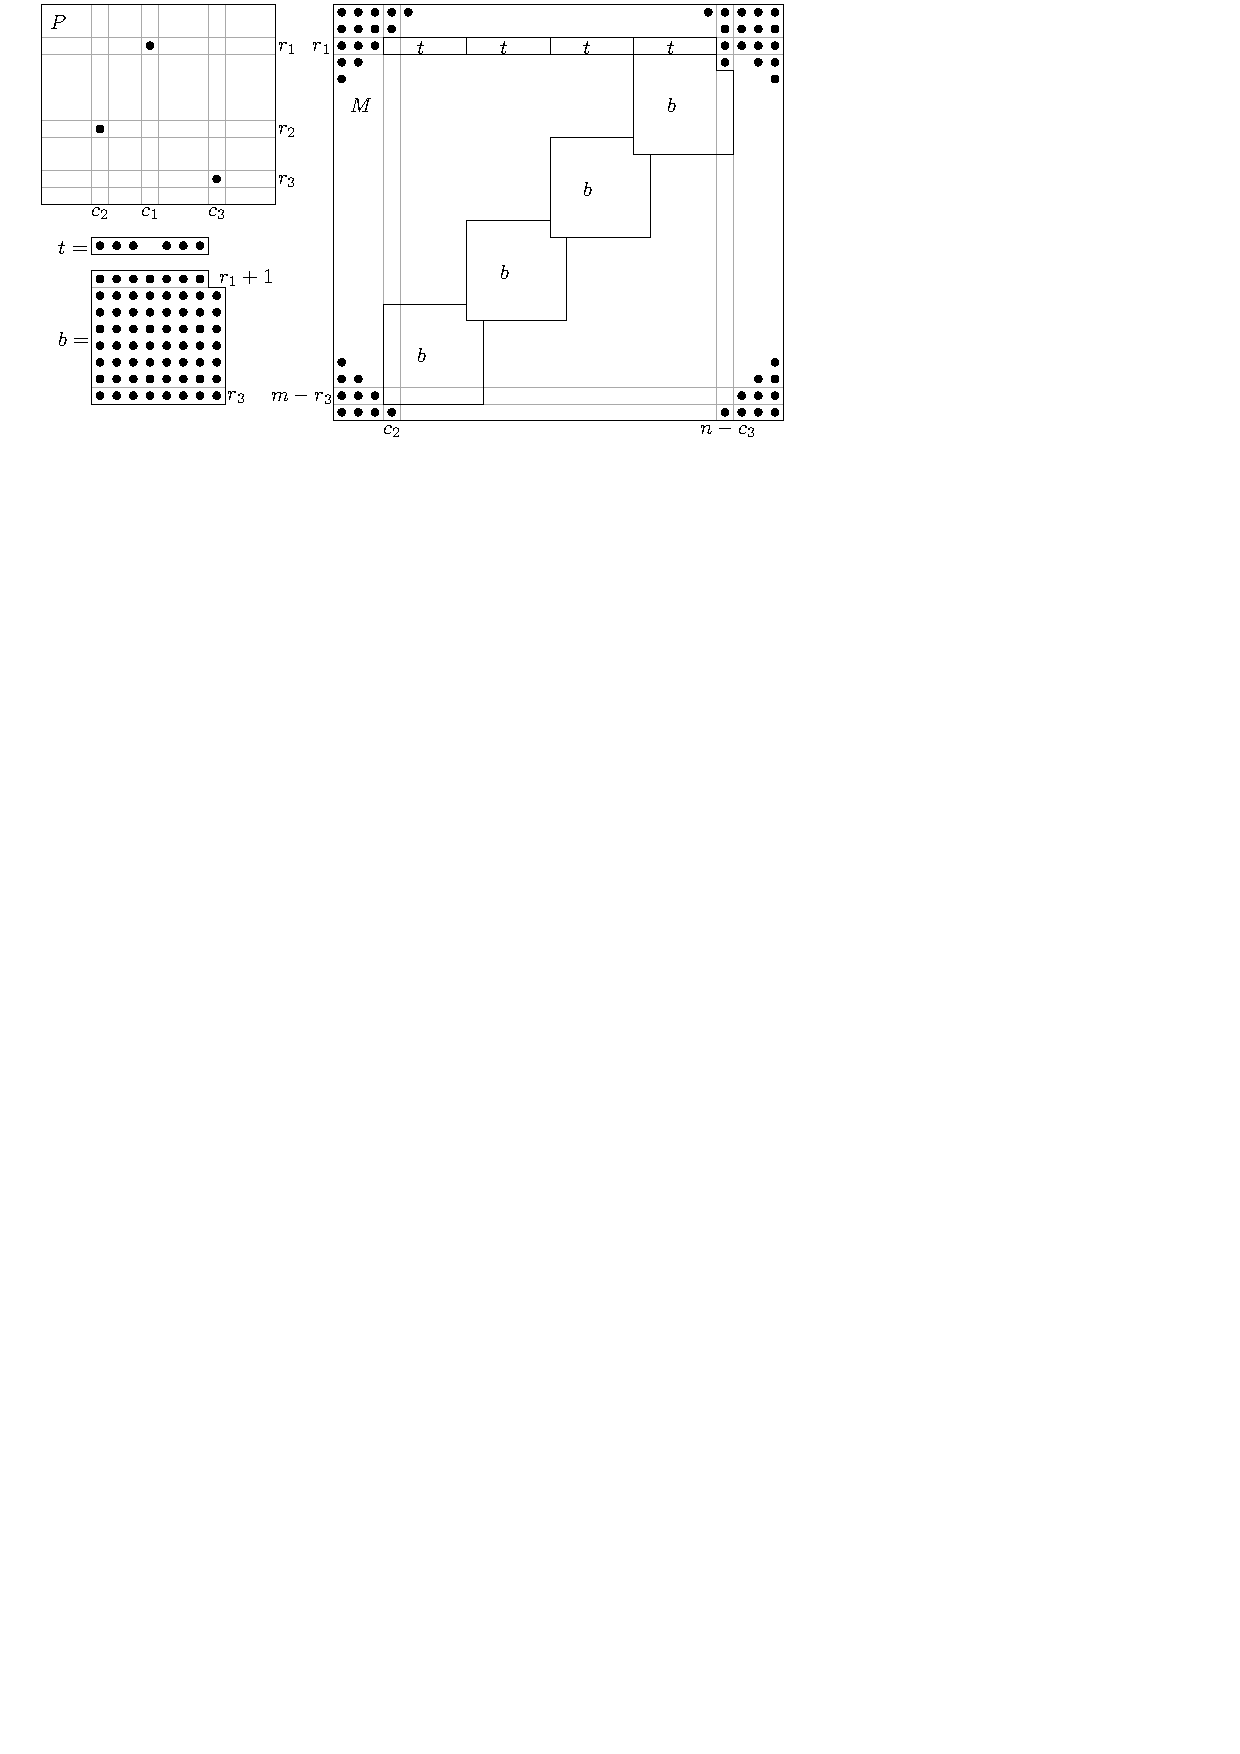
\includegraphics[width=120mm]{img/manyints.pdf}
\caption{The structure of a critical matrix avoiding $P$ that has arbitrarily many zero-intervals.}
\label{fig:manyints}
\end{figure}
\end{proof}

\subsection{Bounding patterns}
\label{subsec:bound}
What makes it even more interesting is that any pattern avoiding all rotations of $P_1$ as interval minors is already bounding. For simplicity, whenever we say that a matrix has only $k$ non-empty lines, we mean that every one-entry belongs to one of the $k$ lines.

\begin{thm}
\label{thm:boundedints}
Let $P$ be a pattern avoiding all rotations of $P_1$, then $P$
\begin{enumerate}
	\item contains at most three non-empty lines or
	\item avoids $\smm{\bullet& \\ &\bullet}$ or $\smm{ &\bullet\\\bullet& }$.
\end{enumerate}
\end{thm}
\begin{proof}
Assume $P$ has four one-entries that do not share any row or column. Then those one-entries induce a $4\times4$ permutation inside $P$ and because $P$ does not contain any rotation of $P_1$, the induced permutation is either $1234$ or $4321$. Without loss of generality, assume it is the first one and denote its one-entries by $e_1,e_2,e_3$ and $e_4$. Clearly, no one-entry from $e_1,e_2,e_3$ and $e_4$ can be part of any mapping of $P'=\smm{\bullet& \\ &\bullet}$ because it would induce a mapping of a rotation of $P_1$.

Let $e_2=P[r_2,c_2]$ and $e_3=P[r_3,c_3]$. The submatrix~$P[[r_2],[c_2,l]]$ avoids $P'$; otherwise, together with $e_1$ it would give $P_2$ as an interval minor. Symmetrically, $P'\nim P[[r_3,k],[c_3]]$. The submatrix~$P[[r_3-1],[c_3-1]]$ is empty; as otherwise, any one-entry would create a rotation of $P_1$ with $e_3$ and either $e_1$ or $e_2$. Symmetrically, the submatrix $P[[r_2-1],[c_2-1]]$ is also empty. This leave no one-entry in $P$ to be used to map $P'[1,1]$ and so $P'\nim P$.
\end{proof}

We now need to prove that whenever $P$ avoids all rotations of $P_1$ (and satisfies one of the conditions we just showed) it is bounding.

%%%%%%%%%%%%%%%%%%%%%%%%%%%%%%%%%%%%%%%%%%%%%%%%%% one non-empty line
\begin{lemma}
Let $P\in\Pat$ be a pattern having one non-empty line. Then $\rc{\Avm{P}}\leq k$ and $\cc{\Avm{P}}\leq l$.
\end{lemma}
\begin{proof}
Without loss of generality, let the non-empty line be a row~$r$. Consider any matrix~$M\in\Avmax{P}$. Submatrices $M[[r-1],[n]]$ and $M[[m-r+1,m],[n]]$ contain no zero-entry. If we look at any other row, it cannot contain $k$ one-entries, so the maximum number of zero-intervals is $k$.

Consider a column~$c$ of $M$. If there is at least one one-entry in $M[[r,m-r-1],c]$ then because $M$ is critical, the whole column is made of one-entries. Otherwise, there are two one-intervals $M[[r-1],c]$ and $M[[m-r,m],c]$.
\end{proof}

%%%%%%%%%%%%%%%%%%%%%%%%%%%%%%%%%%%%%%%%%%%%%%%%%% two non-empty lines
\begin{lemma}
Let $P\in\Pat$ be a pattern having two non-empty lines. Then $\rc{\Avm{P}}\leq k^2+l$ and $\cc{\Avm{P}}\leq l^2+k$.
\end{lemma}
\begin{proof}
First, we assume the two non-empty lines of $P$ are rows $r_1<r_2$ (or symmetrically columns) and consider any matrix~$M\in\Avmax{P}$. From Observation~\ref{obs:emptyrows} and maximality of $M$, we have that the submatrices $M[[r_1-1],[n]]$ and $M[[m-r_2+1,m],[n]]$ contain no zero-entry. Therefore, we may restrict ourselves to the case when $r_1=1$ and $r_2=k$. From Corollary~\ref{cor:twocols}, we have that there are at most $k^2$ zero-intervals in each row of $M$ and there are at most two zero-intervals in each column of $M$.

Let the two non-empty lines of $P$ be a row~$r$ and a column~$c$. Because of symmetry, we only show the bound for rows. For every one-entry~$e$ of $P$, except those in the row~$r$, there is at most one zero-interval usable for $e$ in each row of any $M\Avmax{P}$. For contradiction, assume there are two such zero-intervals $z_1$ and $z_2$ in the same row. Let Figure~\ref{fig:twolines} illustrate the situation where red and blue lines form two mappings of $P$ to $M$ when a zero-entry of $z_1$ and $z_2$ respectively is changed to a one-entry used to map $e$. When we take the outer two vertical and horizontal lines, we get a mapping of $P$ that uses an existing one-entry in between $z_1$ and $z_2$ to map $e$. This is a contradiction with $\PnimM$.

\begin{figure}[!ht]
\centering
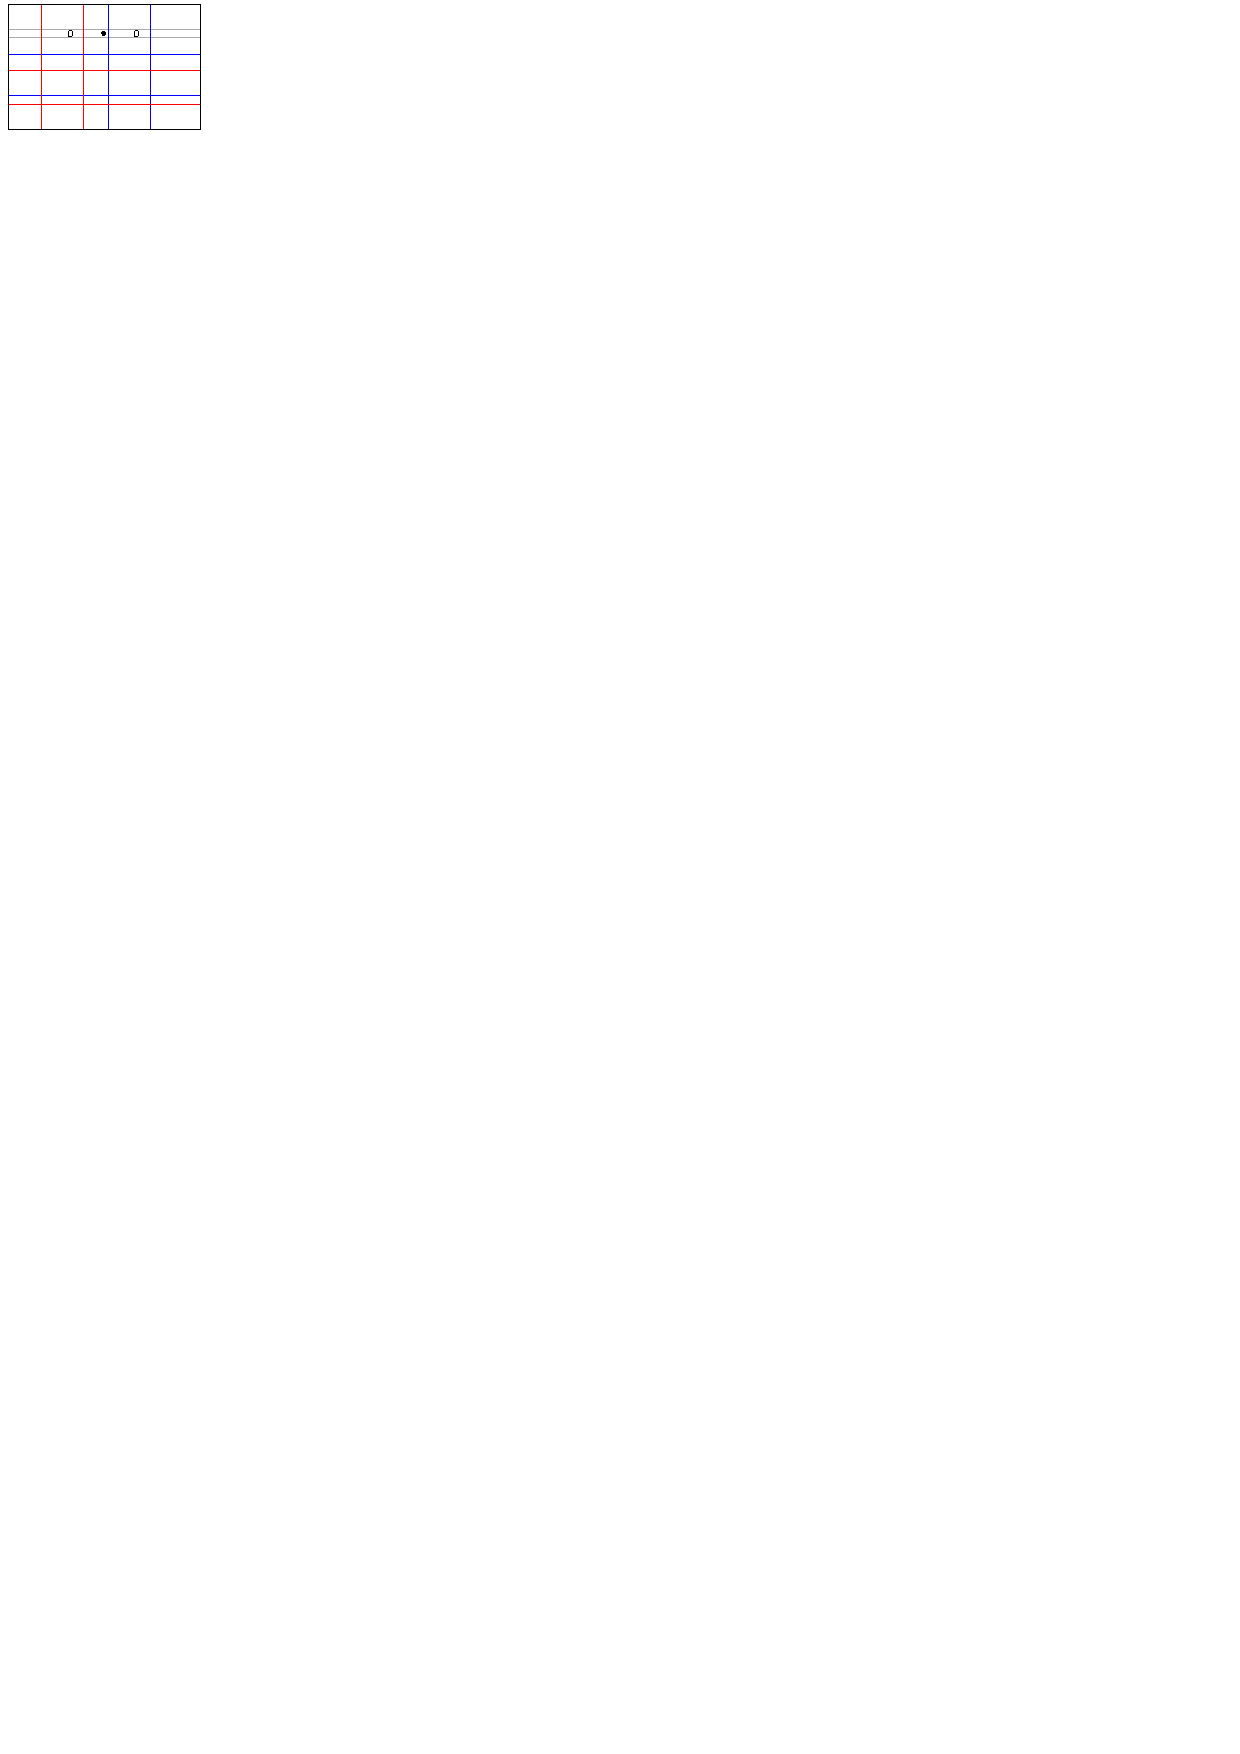
\includegraphics[width=65mm]{img/twolinescol.pdf}
\caption{Red and blue lines representing two different mappings of a forbidden pattern. The two horizontal lines show the boundaries of the mapping of row~$r$ and the vertical lines show the boundaries of the mapping of column~$c$.}
\label{fig:twolines}
\end{figure}

For a one-entry $e=P[r,c']$, if $c'\leq c$ then there must be less than $c'$ one-entries before any zero-intervals usable for $e$; otherwise, we could map $P[r,[1,c']]$ just to the single row of $M$. It follows that $e$ is row-bounded. Symmetrically, the same holds in case $c'>c$ and together we have at most $k+l$ zero-intervals in each $M\in\Avmax{P}$.
\end{proof}

Before we proof the other cases, let us introduce three useful lemmata that make the future case analysis bearable.

%%%%%%%%%%%%%%%%%%%%%%%%%%%%%%%%%%%%%%%%%%%%%% Lemma H
\begin{lemma}
\label{lemma:H}
Let $P\in\Pat$ be one of the four matrices in Figure~\ref{fig:lemmaH}. Then every one-entry in $P[\{r_2\},[c_1,c_2]]$ is row-bounded. Moreover, the same also holds if we change some one-entries to zero-entries.

\begin{figure}[!ht]
\centering
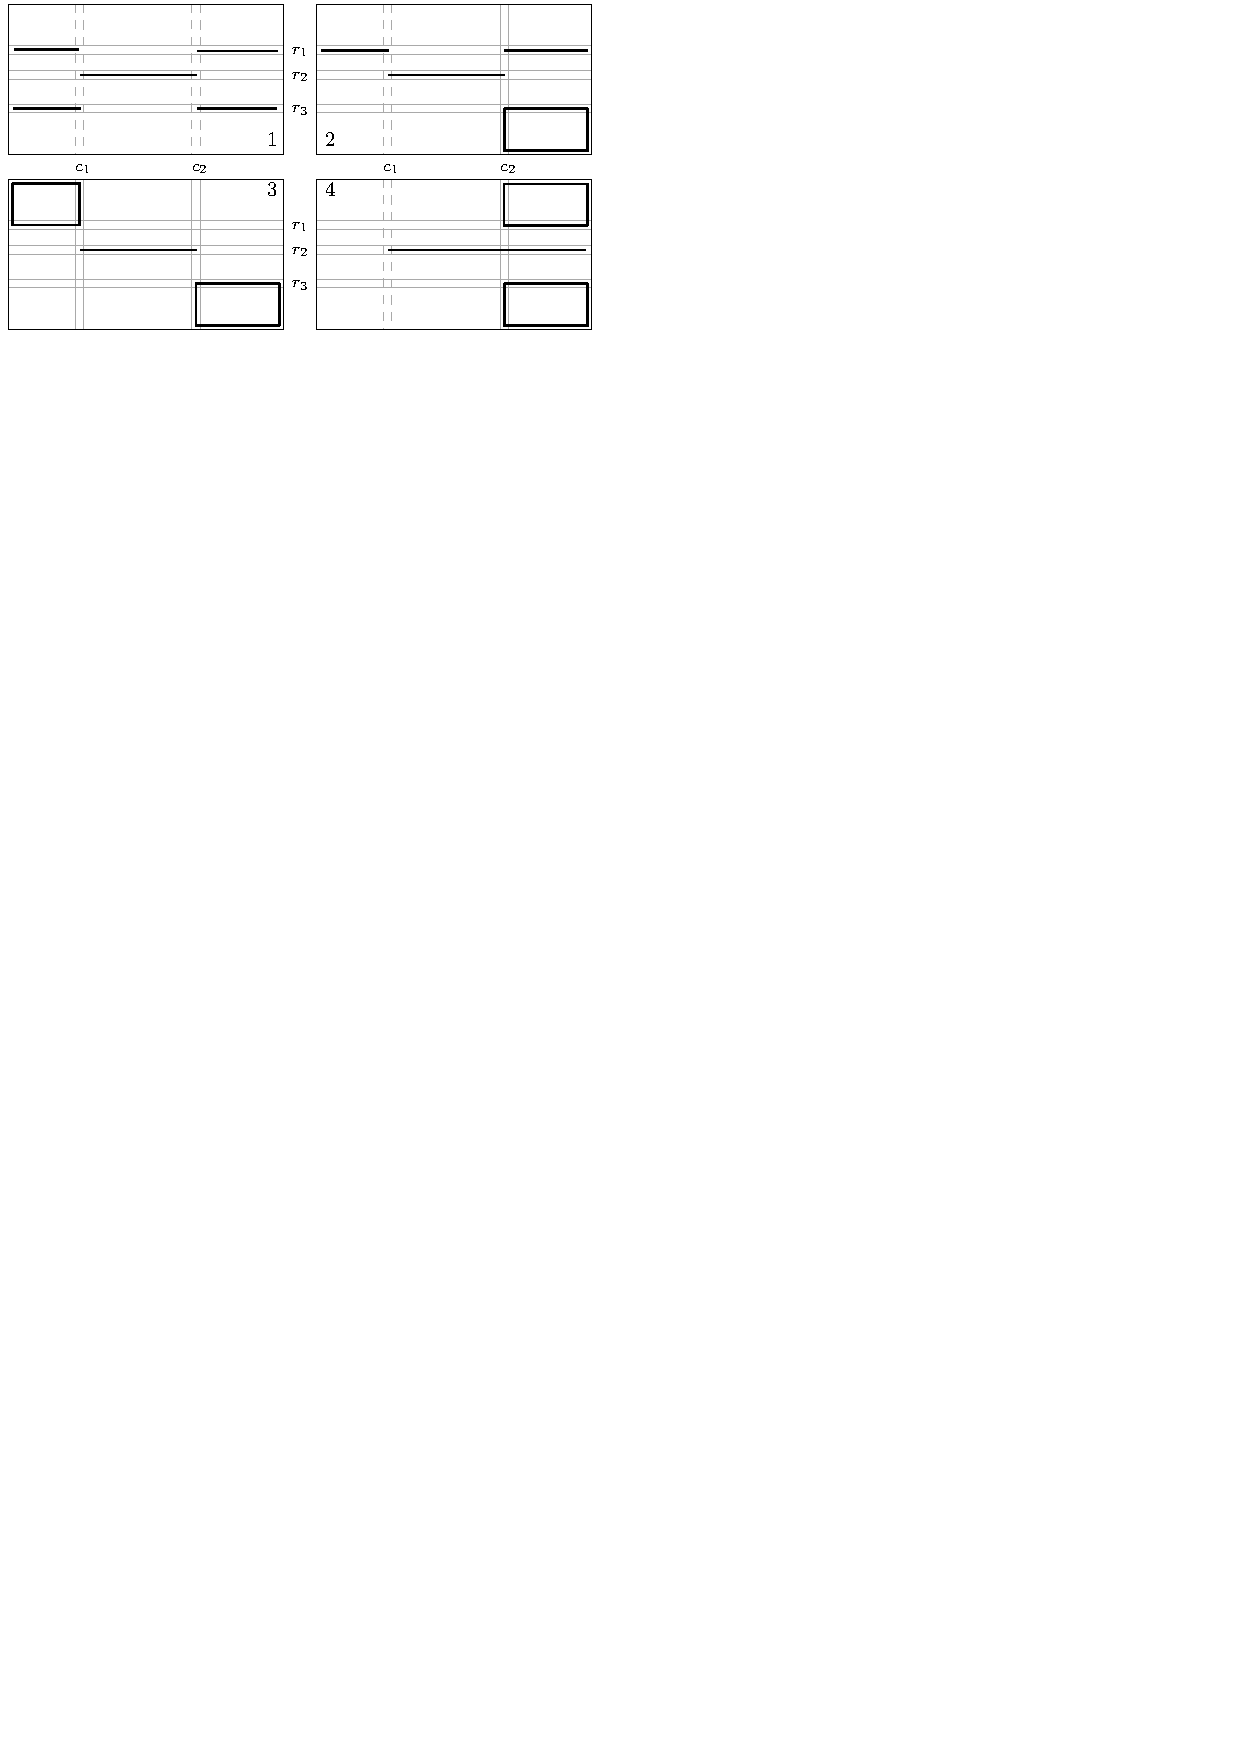
\includegraphics[width=\textwidth]{img/lemmaH.pdf}
\caption{The patterns for which all one-entries in the row~$r_2$ and the columns $[c_1,c_2]$ are row-bounded. One-entries of the patterns are inside the bold rectangles and on the bold lines.}
\label{fig:lemmaH}
\end{figure}
\end{lemma}
\begin{proof}
Let a pattern~$P$ be the first described matrix and let $k'=c_2-c_1$. We show that for each one-entry~$e\in P[\{r_2\},[c_1,c_2]]$ and every matrix~$M\in\Avmax{P}$ there are at most $k'$ zero-intervals usable for $e$ in each row of $M$. For contradiction, assume there is a row~$r$ with $k'+1$ zero-intervals usable for some $e$. It follows that there are at least $k'$ one-entries in between the two most distant zero-intervals $z_1$ and $z_2$. Therefore, the whole row~$r_2$ can be mapped just to the row~$r$. Changing a zero-entry of $z_1$ to a one-entry, to which $e$ can be mapped, creates a mapping of $P$ to $M$, in which all one-entries from columns $[c_1]$ are mapped to columns before $z_1$ (and $z_1$) and similarly all one-entries from columns $[c_2,l]$ can be mapped to columns past $z_2$ (and $z_2$). It also holds that all the one-entries from the row~$r_1$ are mapped (in both mappings) to one-entries of $M$ in rows $[r-r_2+r_1]$ (and symmetrically for one-entries from the row~$r_3$). Thus, we can simply map empty rows $[r_1+1,r_3-1]$ around row $r$ and use the rest to map rows $r_1$ and $r_2$.
%The described mapping gives us $\PimM$ and a contradiction. We can see the mapping in Figure~\ref{fig:lemmaH1}.
%\begin{figure}[!ht]
%\centering
%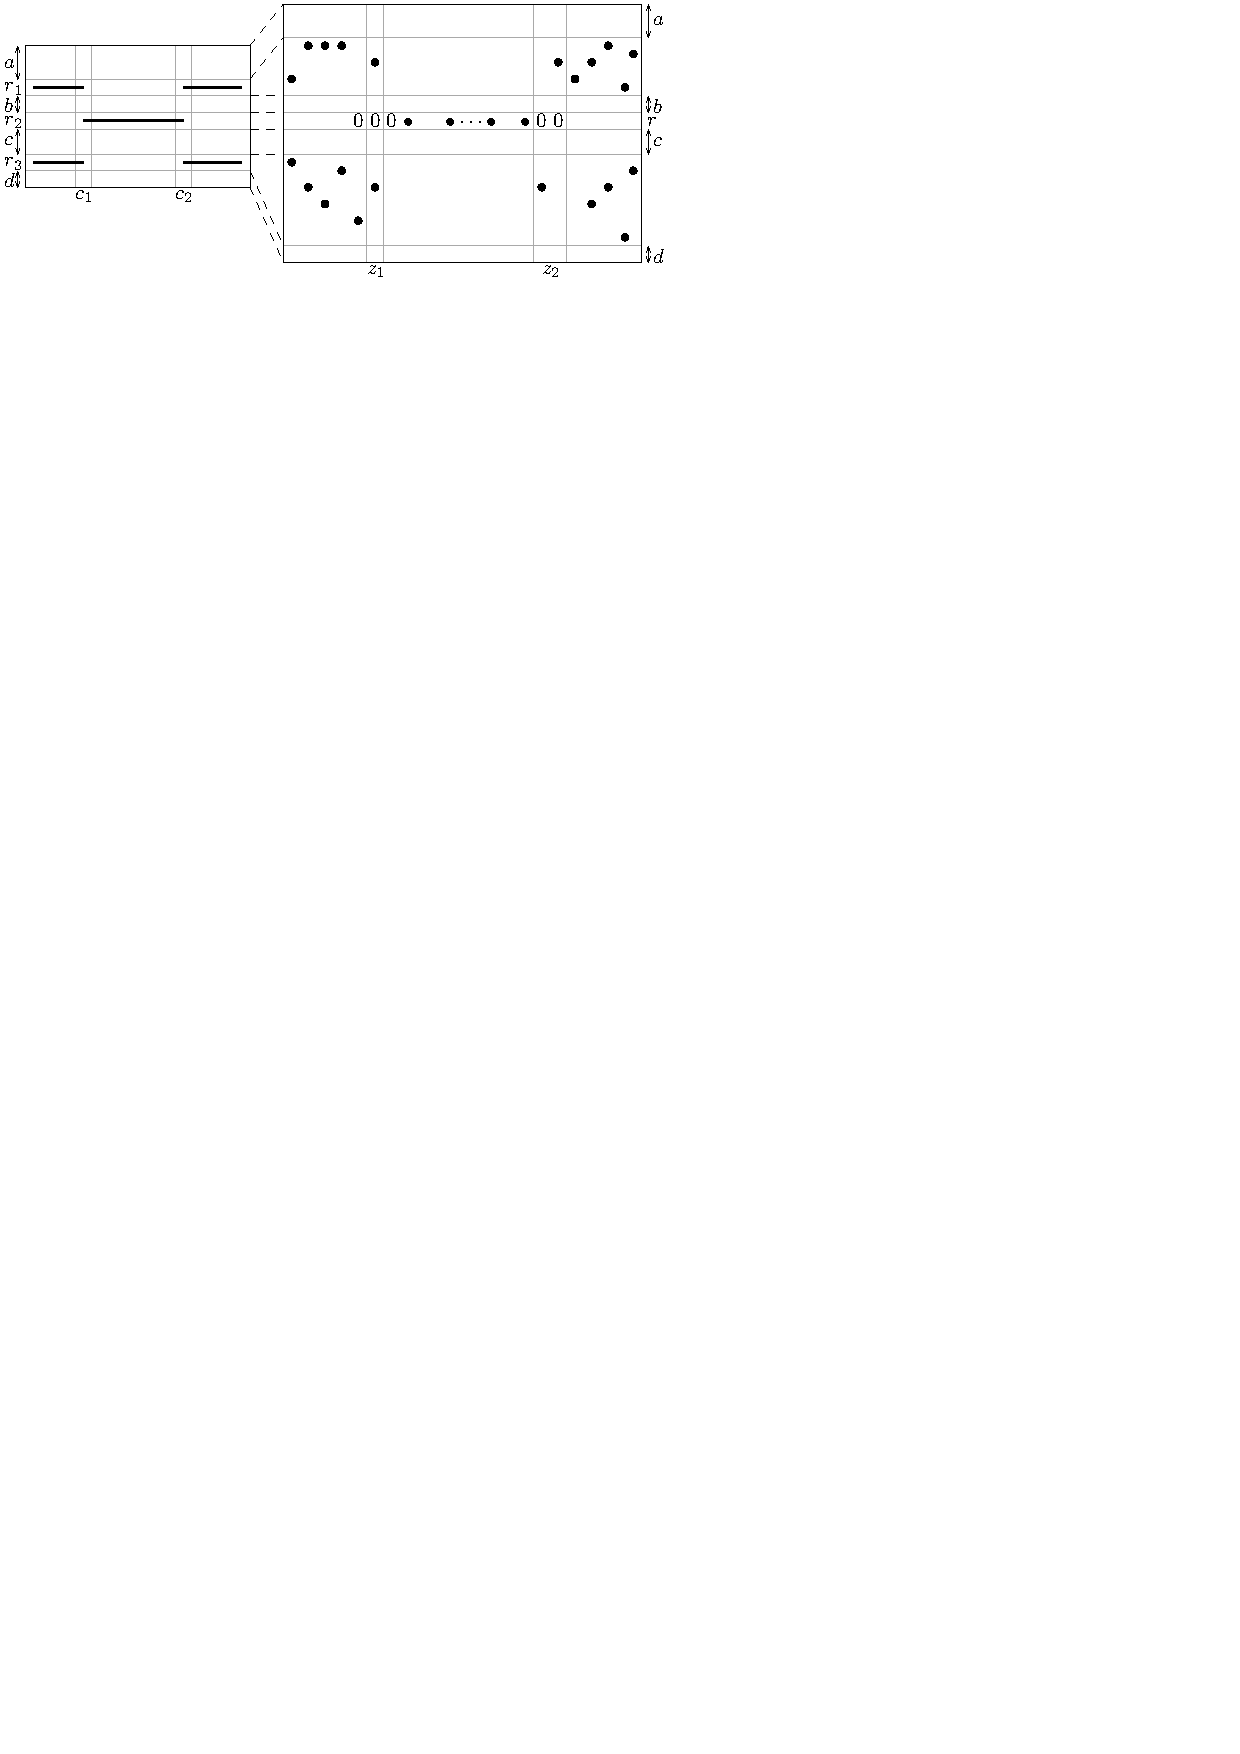
\includegraphics[width=\textwidth]{img/lemmaH1.pdf}
%\caption{Mapping of a pattern into a matrix only using one line to map an empty line of the pattern and only using one line to map row~$r_2$.}
%\label{fig:lemmaH1}
%\end{figure}

Proofs of cases two and three are similar to the first one and we skip them.

Let a pattern~$P$ be the fourth described matrix and consider any matrix~$M\in\Avmax{P}$. For the $i$-th one-entry~$e$ in the row~$r_2$ (ordered from left to right and only considering those in columns $[c_1,c_2]$) no zero-interval of $M$ usable for $e$ cannot have $i$ one-entries before it and so the row-complexity of each such one-entry is bounded by $i\geq l$.

Throughout the proof, we have never used as a fact that an entry of $M$ is a one-entry and so the proof also holds for any pattern~$P$ created from any of the fourth described matrices by deletion of one-entries.
\end{proof}

It is important to realize that we could not have used the same proof we used for the first three cases also for the fourth case, because we can never rely on the fact a mapping of $P$ only uses one row of $M$ to map the row~$r_2$. This is because in the fourth case, there are also potential one-entries in $P[\{r_2\},[c_2+1,l]]$.

What follows is a direct corollary of the fourth case of just stated Lemma~\ref{lemma:H}. Even though it is very simple and straightforward, it is going to be used so often that it is worth stating it apart from the rest.

%%%%%%%%%%%%%%%%%%%%%%%%%%%%%%%%%%%%%%%%%%%%%% First non-empty column bounded
\begin{lemma}
\label{lemma:First}
Let $P$ be a matrix and let $c$ be its first non-empty column. Then every one-entry from $c$ is row-bounded. \qed
\end{lemma}

%%%%%%%%%%%%%%%%%%%%%%%%%%%%%%%%%%%%%%%%%%%% Lemma I
\begin{lemma}
\label{lemma:I}
Let $P\in\Pat$ be one of the three matrices in Figure~\ref{fig:lemmaI}. Then every one-entry in $P[[r_1+1,r_2-1],\{c\}]$ is row-bounded. Moreover, the same also holds if we change some one-entries to zero-entries.

\begin{figure}[!ht]
\centering
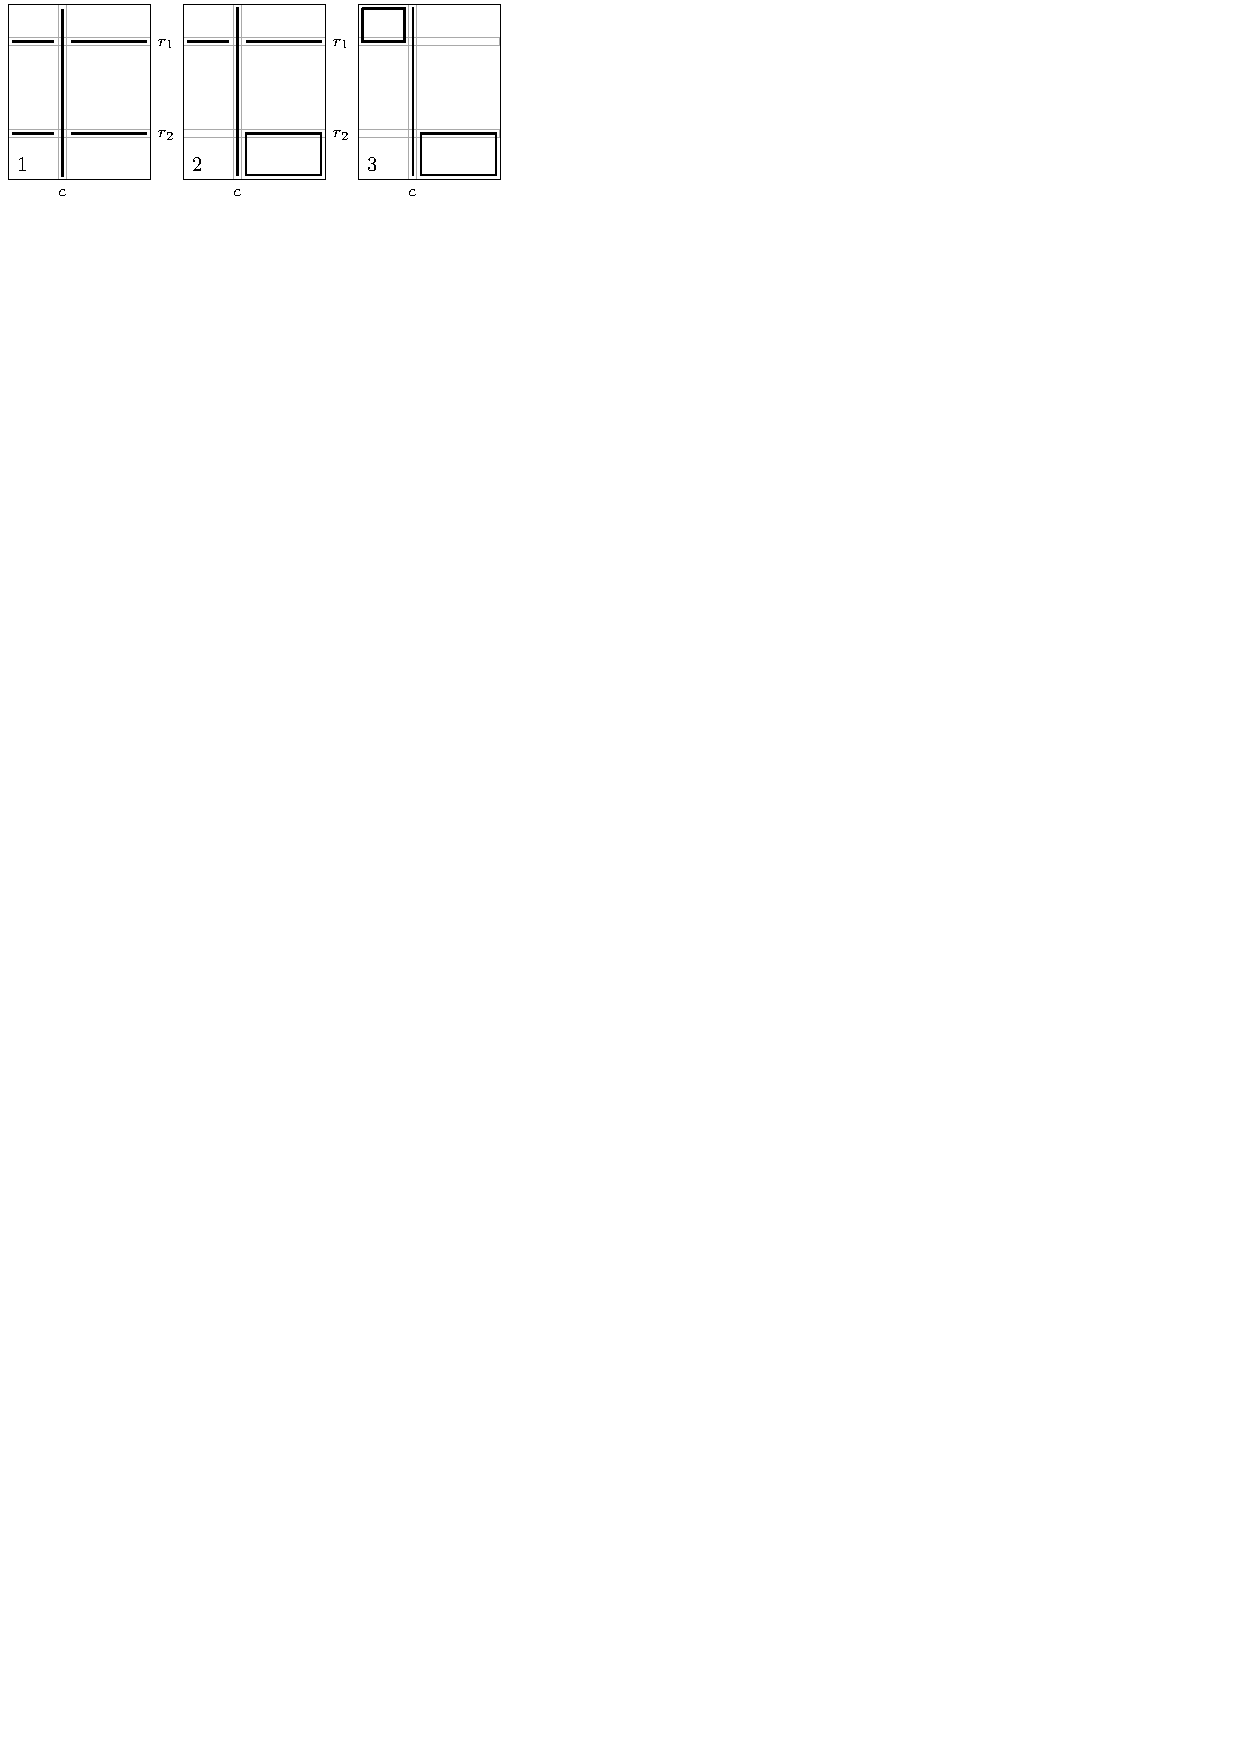
\includegraphics[width=120mm]{img/lemmaI.pdf}
\caption{The patterns for which all one-entries in the column~$c$ and the rows~$[r_1+1,r_2-1]$ are row-bounded. One-entries of the patterns are inside the bold rectangles and on the bold lines.}
\label{fig:lemmaI}
\end{figure}
\end{lemma}
\begin{proof}
Let $P$ be a submatrix of the first described matrix. We show that for each one-entry~$e$ from $P[[r_1+1,r_2-1],\{c\}]$ and every matrix $M\in\Avmax{P}$ there is at most one zero-interval usable for $e$ in $M$. For contradiction, assume there is a row~$r$ with two zero-intervals $z_1$ and $z_2$ usable for $e$. Consider Figure~\ref{fig:lemmaI1}, where the red lines show a mapping of $P$ to $M$ created when a zero-entry of $z_1$ is changed to a one-entry used to map $e$ and the blue lines show a mapping of $P$ to $M$ created when a zero-entry of $z_2$ is changed to a one-entry used to map $e$. If we map the column~$c$ to the columns of $M$ enclosed by the two outer vertical lines and map rows $r_1$ and $r_2$ again to rows enclosed by the corresponding two outer horizontal lines, we get a mapping of $P$ to $M$ and so a contradiction with $\PnimM$.

\begin{figure}[!ht]
\centering
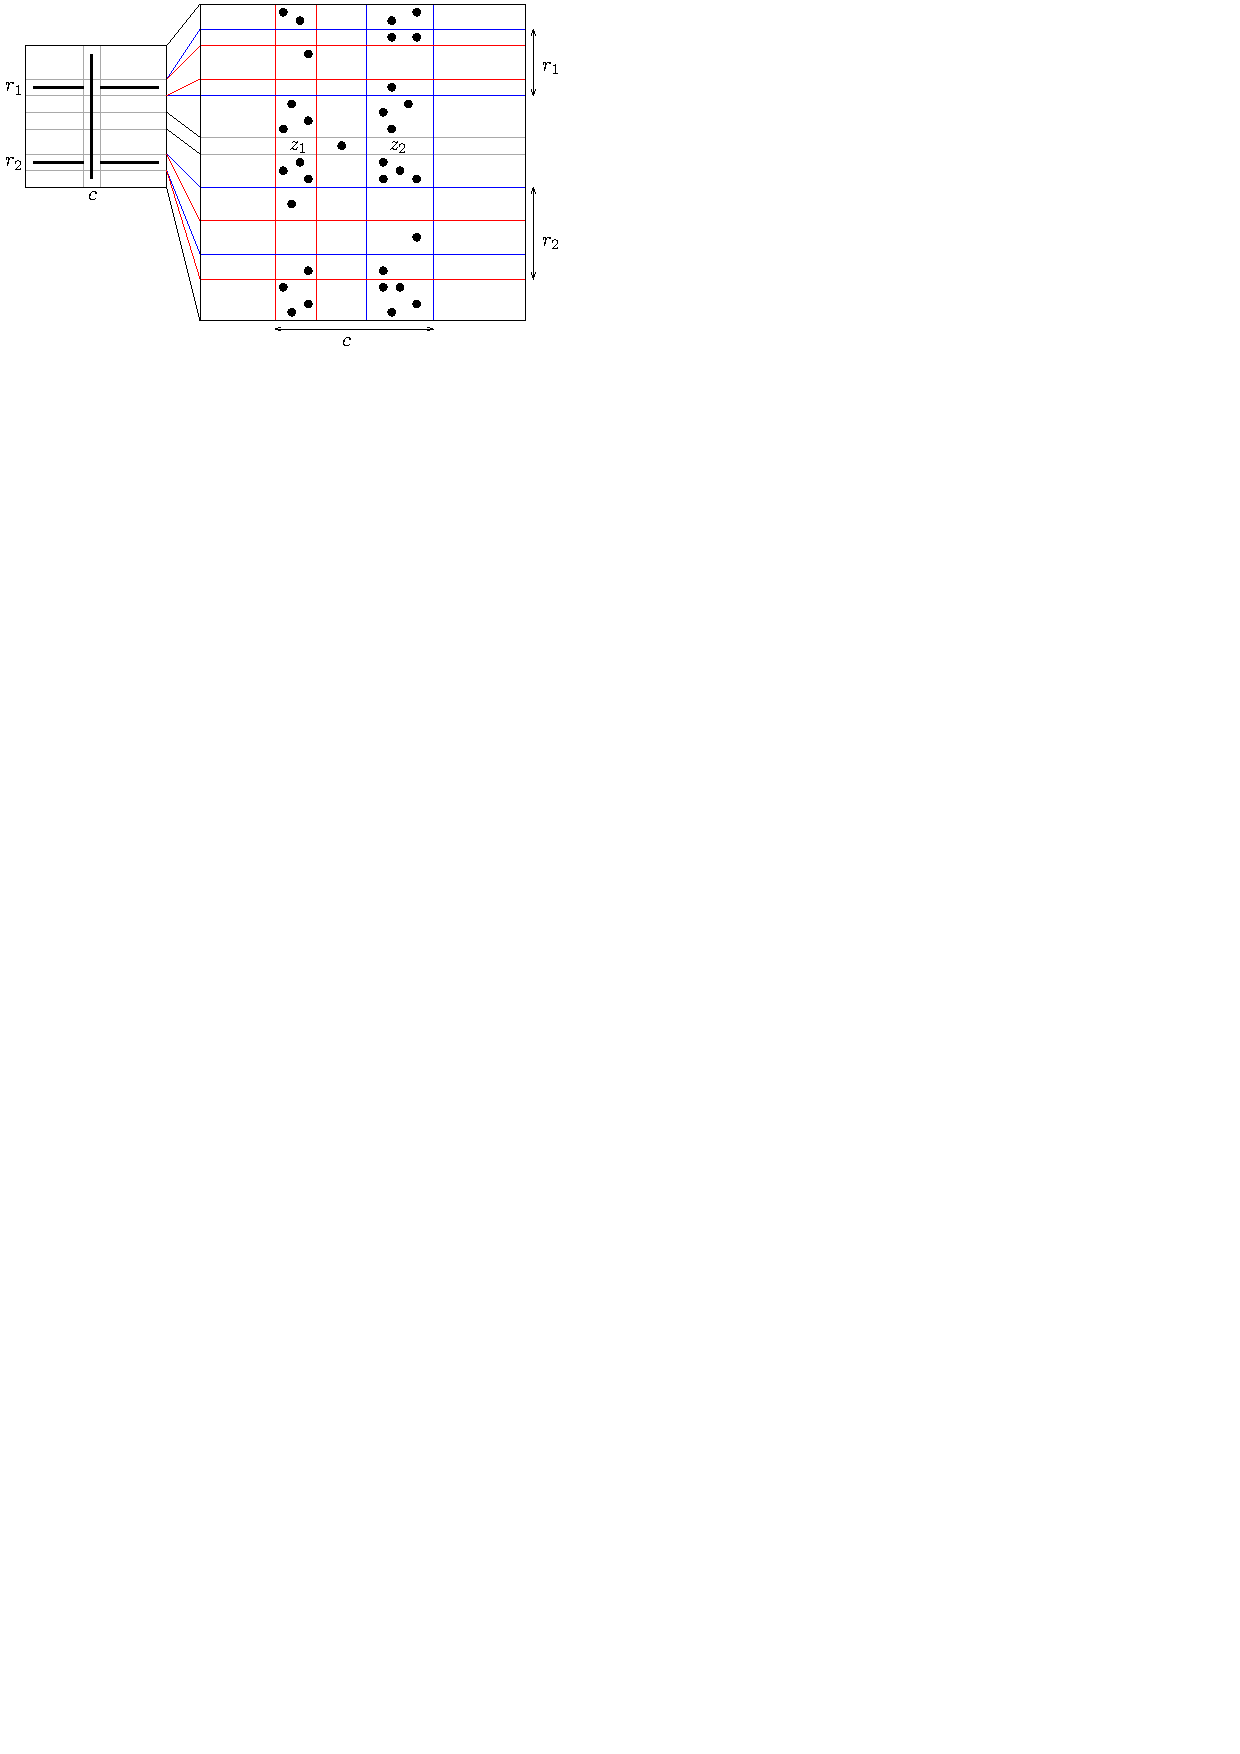
\includegraphics[width=100mm]{img/lemmaI1col.pdf}
\caption{Red and blue lines representing two different mappings of a forbidden pattern. The four horizontal lines show the boundaries of the mapping of rows~$r_1$ and $r_2$ and the vertical lines show the boundaries of the mapping of the column~$c$.}
\label{fig:lemmaI1}
\end{figure}
Proofs of cases two and three are similar to the first one and we skip them.

Throughout the proof, we have never used as a fact that an entry of $M$ is a one-entry and so the proof also holds for any pattern~$P$ created from any of the fourth described matrices by deletion of one-entries.
\end{proof}

\begin{lemma}
\label{lemma:I2}
Let a pattern~$P\in\Pat$ be created from one of the matrices in Figure~\ref{fig:lemmaI2} by deletion of one-entries and let $c=l-1$. Then every one-entry in $P[[r_1,r_2],\{c\}]$ is row-bounded.

\begin{figure}[!ht]
\centering
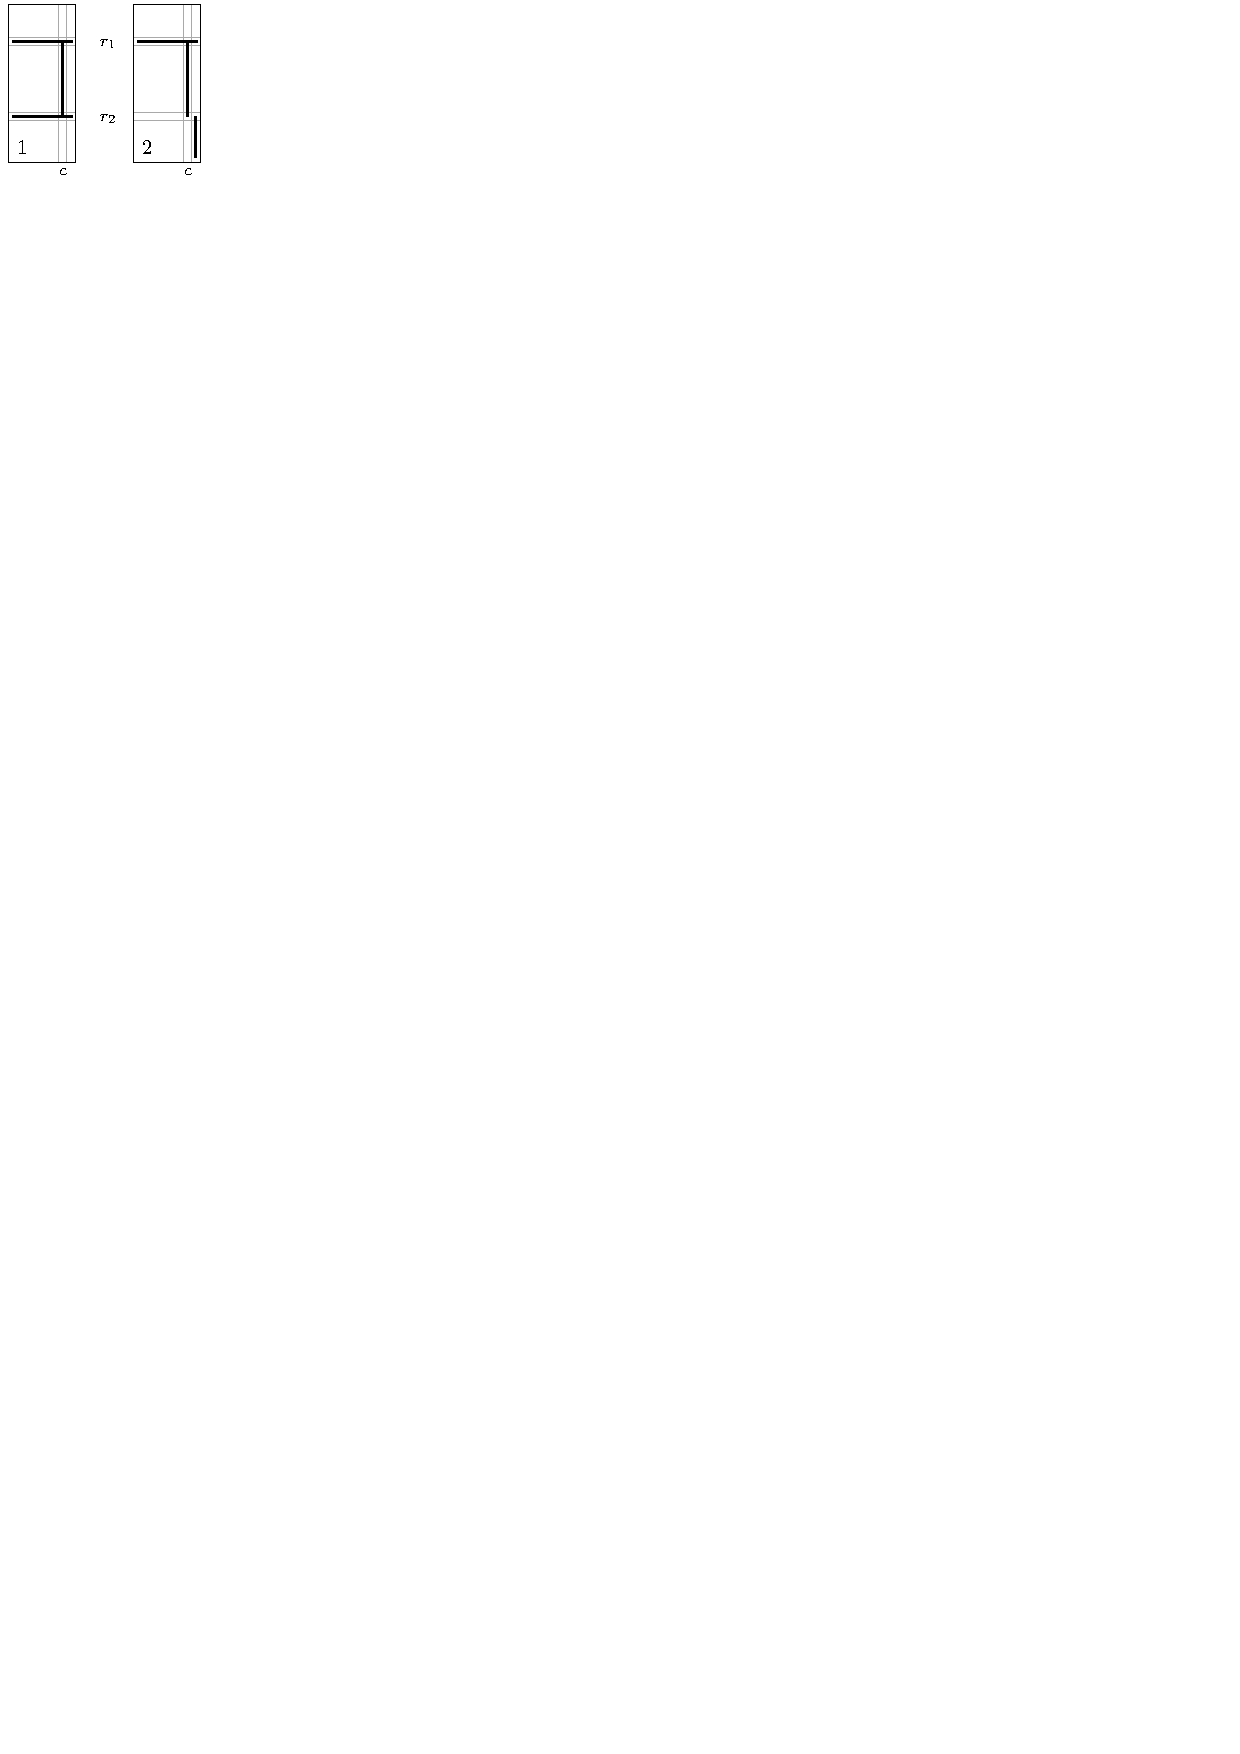
\includegraphics[width=45mm]{img/lemmaI2.pdf}
\caption{The patterns for which all one-entries in the column~$c$ and the rows~$[r_1,r_2]$ are row-bounded. One-entries of the patterns are on the bold lines and the column $c$ is the second last.}
\label{fig:lemmaI2}
\end{figure}
\end{lemma}
\begin{proof}
Let a pattern~$P$ be created from the first described matrix. From~\ref{lemma:I}, we know that all one-entries in $P[[r_1+1,r_2-1],\{c\}]$ are row-bounded. Thank to symmetry, it suffices to show that the one-entry~$e=P[r_1,c]$ is row-bounded. Without loss of generality, we have $P[r_2,l]=1$; otherwise, we can use the fourth case of Lemma~\ref{fig:lemmaH} to prove that $e$ is row-bounded.

Consider any matrix~$M\in\Avmax{P}$ and let $z_1<z_2$ be any two zero-intervals from the same row usable for $e$. Without loss of generality, in any mapping of $P$ to $M$, created when a zero-entry of $z_1$ is changed to a one-entry used to map $e$, the one-entry~$P[r_2,l]$ is mapped to a column before $z_2$. Otherwise, if we map $e$ to the one-entry between $z_1$ and $z_2$ and map $P[r_1,l]$ to any one-entry behind $z_2$ we get a mapping showing $P\im M$.

We prove there are at most $l$ zero-intervals usable for $e$ on every row of $M$. For contradiction, let there be such zero-intervals $z_1,\dots,z_l$ that there is a one-entry behind each of them. For each zero-interval $z_i$, let $e_i$ be any one-entry of $M$ that can be used to map the one-entry~$P[r_2,l]$ if a zero-entry of $z_i$ is changed to a one-entry used to map $e$. In the sequence $e_1,\dots,e_l$ there either are two one-entries $M[r'_1,c'_1],M[r'_2,c'_2]$ such that $r'_1\leq r'_2$, or the rows of one-entries form a decreasing sequence.

Let us first consider the first case and let $e_i=M[r'_1,c'_1]$ and $e_j=M[r'_2,c'_2]$. Consider a mapping of $P$ to $M$ created when a zero-entry of $z_i$ is changed to a one-entry used to map $e$. If in this mapping, we map $e$ to a one-entry between $z_i$ and $z_j$, map $P[r_1,l]$ to a one-entry behind $z_j$, map $P[r_2,l-1]$ to $e_i$ and map $P[r_2,l]$ to $e_j$, we get a mapping of $P$ to $M$, which is a contradiction.

And so it holds that the one-entries $e_1,\dots,e_l$ form a row decreasing sequence. We can pair every $e_i$ with a one-entry bounding $z_i$ from the right and so we can map the whole submatrix $P[[k],[l-2]]$ just to columns before $z_{l-1}$ of $M$. Because $z_l$ is usable for $e$, there are enough one-entries to map the whole column~$c$ there and there are one-entries where $P[r_1,l]$ and $P[r_2,l]$ can be mapped. The only problem is that $e$ is mapped to a one-entry created by changing a zero-entry of $z_l$ but we can also map it to a one-entry between zero-intervals $z_{l-1}$ and $z_l$ and we have $P\im M$ and a contradiction.\\

Let a pattern~$P$ be created from the second described matrix. All one-entries in $P[[r_1+1,r_2-1],\{c\}]$ are row-bounded thanks to (the second case of) Lemma~\ref{lemma:I}. From the fourth case of Lemma~\ref{lemma:H}, the one-entry~$P[r_1,c]$ is also row-bounded. So we only need to prove that the one-entry~$P[r_2,c]$ is row-bounded.

Without loss of generality, $P[r_1,l]=1$; otherwise, $\smm{ &\bullet\\\bullet& }\nim P$ and in the following Lemma~\ref{lemma:walkpat}, we show that every such $P$ is bounding. We once again define one-entries $e_1,\dots,e_l$ and use the same analysis as we did in the first case.
\end{proof}

Now that the very technical lemmata are stated, we just use them to easily prove that the remaining patterns described in Theorem~\ref{thm:boundedints} are also bounding.

%%%%%%%%%%%%%%%%%%%%%%%%%%%%%%%%%%%%%%%%%% walking patterns
\begin{lemma}
\label{lemma:walkpat}
Let $P\in\Pat$ be a pattern avoiding $\smm{ &\bullet\\\bullet& }$ or $\smm{\bullet& \\ &\bullet}$. Then $P$ is bounding.
\end{lemma}
\begin{proof}
From Proposition~\ref{prop:walking}, we know that $P$ is a walking pattern. Every one-entry of $P$ satisfies either conditions of the third case of Lemma~\ref{lemma:H} or it satisfies conditions of the third case of Lemma~\ref{lemma:I} and therefore is row-bounded. From Observation~\ref{obs:transposebounded}, we know it is also column-bounded.
\end{proof}

What follows is the last and the most difficult case of our analysis. Its length is caused by the fact that it is harder to describe symmetries than it is to just use the previous lemmata to show that each pattern is bounding.

%%%%%%%%%%%%%%%%%%%%%%%%%%%%%%%%%%%%%%%%%%% three non-empty lines
\begin{lemma}
Let $P\in\Pat$ be a pattern having three non-empty lines and avoiding all rotations of $P_1$. Then $P$ is bounding.
\end{lemma}
\begin{proof}
First of all, if $P$ avoids $\smm{ &\bullet\\\bullet& }$ or $\smm{\bullet& \\ &\bullet}$, we use Lemma~\ref{lemma:walkpat}.

Let the three non-empty lines be three rows and let a pattern~$P$ have one-entries in at least three columns. Then it contains a $3\times3$ permutation matrix as a submatrix. Since the rotations of $P_1$ are avoided, the only feasible permutations are 123 and 321 and without loss of generality, we assume the first case. In Figure~\ref{fig:threelines} we see the structure of $P$. The capital letters stand for one-entries of the permutation and are chosen to be the left-most possible, letters $a-f$ stand each for a potential one-entry and the Greek letters stand each for a potential sequence of one-entries. Everything else is empty. Not all one-entries can be there at the same time, because that would create a mapping of $P_1$ or its rotation. We also need to find $\smm{\bullet& \\ &\bullet}\im P$. The following analysis only uses hereditary arguments, which means that if we prove that $P$ is bounding, we also prove that each submatrix of $P$ is bounding. With this in mind, we restrict ourselves to critical patterns.
\begin{figure}[!ht]
	\centering
	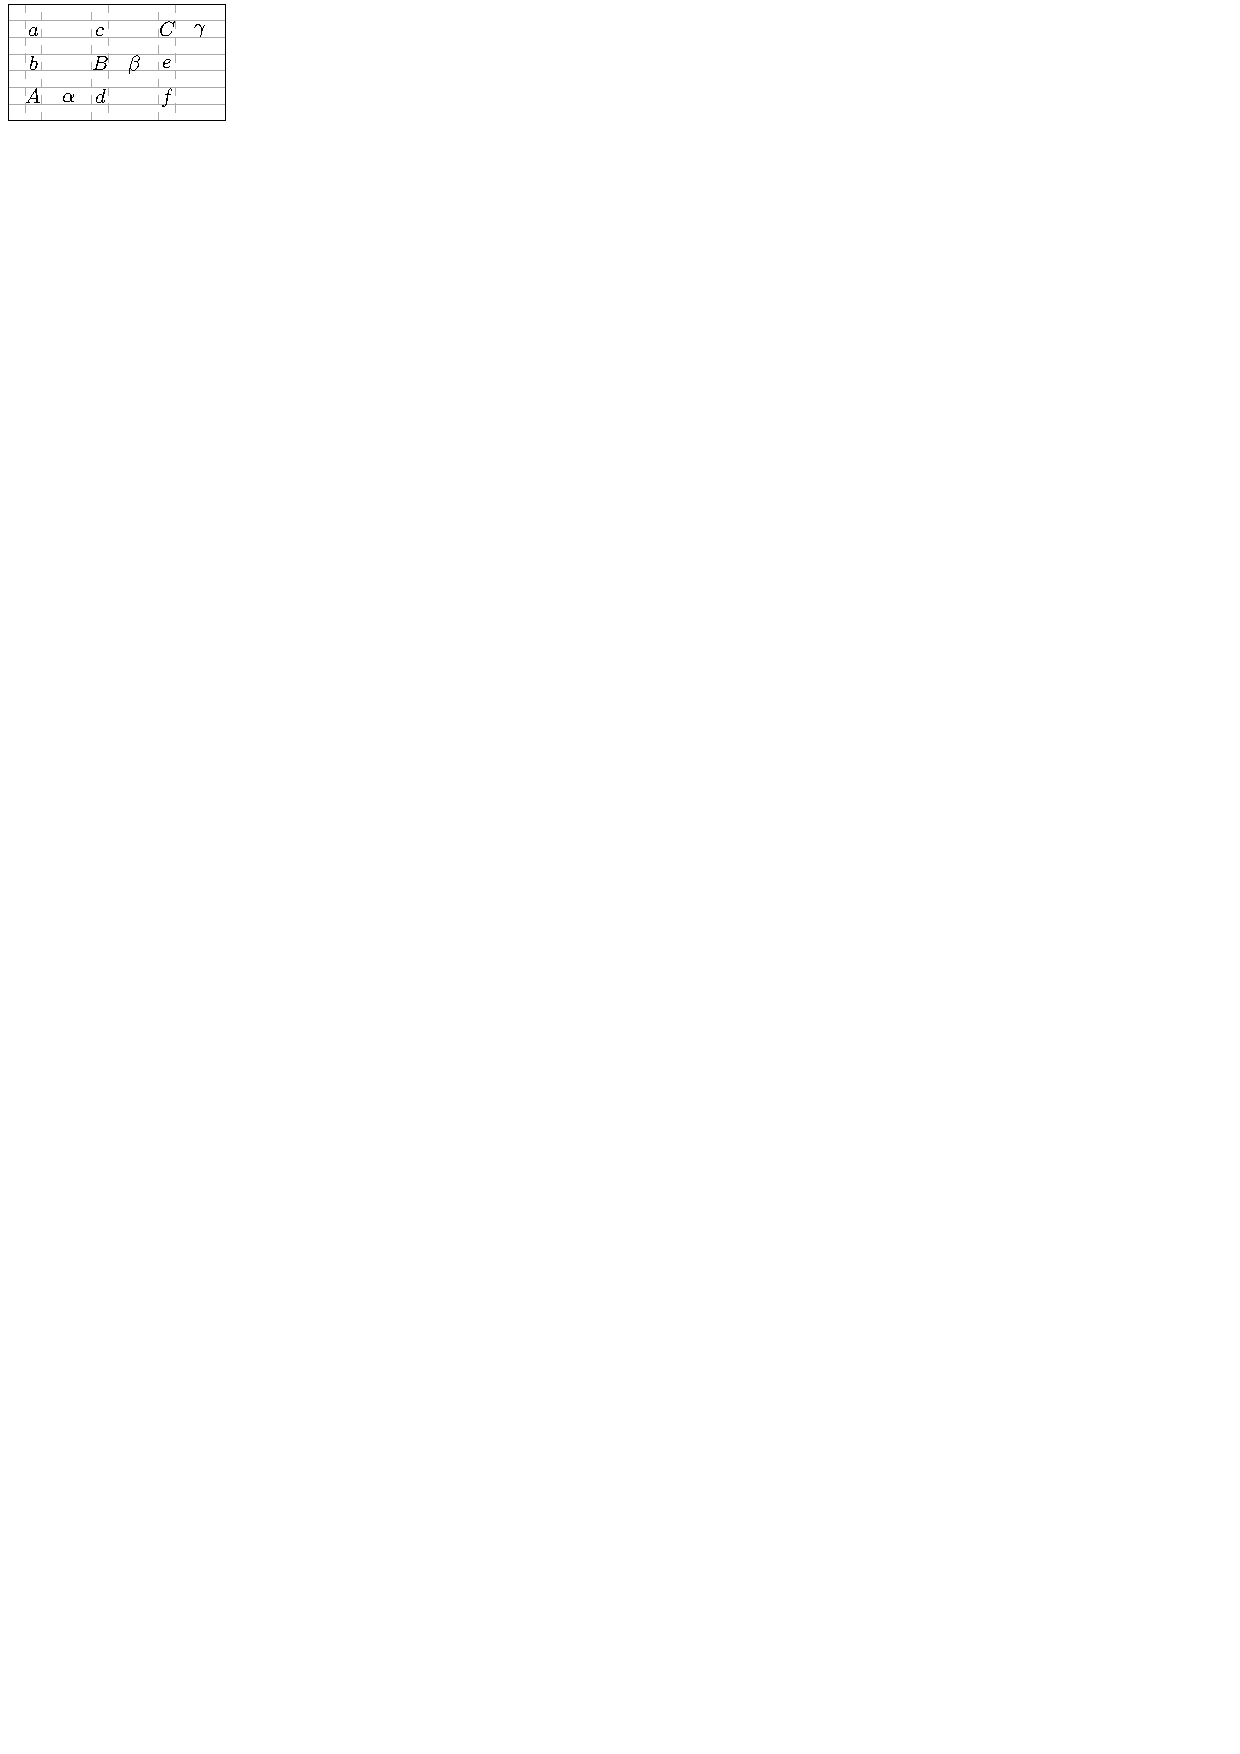
\includegraphics[width=65mm]{img/threelines.pdf}
	\caption{The structure of a pattern only having three non-empty rows and avoiding all rotations of $P_1$.}
	\label{fig:threelines}
\end{figure}
\begin{enumerate}
	\item $\gamma=1\Rightarrow f=0\Rightarrow$ because $\smm{\bullet& \\ &\bullet}\im P$, it holds $a=1\Rightarrow\alpha=0$
		\begin{enumerate}
			\item $d=1\Rightarrow b=0,\ \beta=0,\ e=0$
			\item $d=0$
				\begin{enumerate}
					\item $c=1\Rightarrow\beta=0,\ e=0$
					\item $c=0$
				\end{enumerate}
		\end{enumerate}
	\item $\gamma=0$
		\begin{enumerate}
			\item $\alpha=1\Rightarrow a=0,\ b=0$. If $f=0$ we have case 1. (b) ii.; otherwise, we have case 1. (a).
			\item $\alpha=0$
				\begin{enumerate}
					\item $c=1,\ d=1\Rightarrow b=0,\ e=0,\ \beta=0$
					\item $c=1,\ d=0\Rightarrow e=0,\ \beta=0$ and without loss of generality, $b=1$. Otherwise, we have the previous case. Therefore, $f=0$
					\item $c=0,\ d=1\Rightarrow b=0$. Without loss of generality, $e=1,\ \beta=1$. Otherwise, we have the case $c=1,\ d=1$. Therefore, $a=0$
					\item $c=0,\ d=0$
				\end{enumerate}
		\end{enumerate}
\end{enumerate}
The same analysis also proves that if a pattern with the same restrictions only has three non-empty columns then it is bounding.

Let $P$ be a pattern having two non-empty rows~$r_1,r_2$ and one non-empty column~$c_1$. Without loss of generality, we again assume permutation 123 is present and we distinguish three cases. Consider Figure~\ref{fig:twoplusone}:
\begin{figure}[!ht]
	\centering
	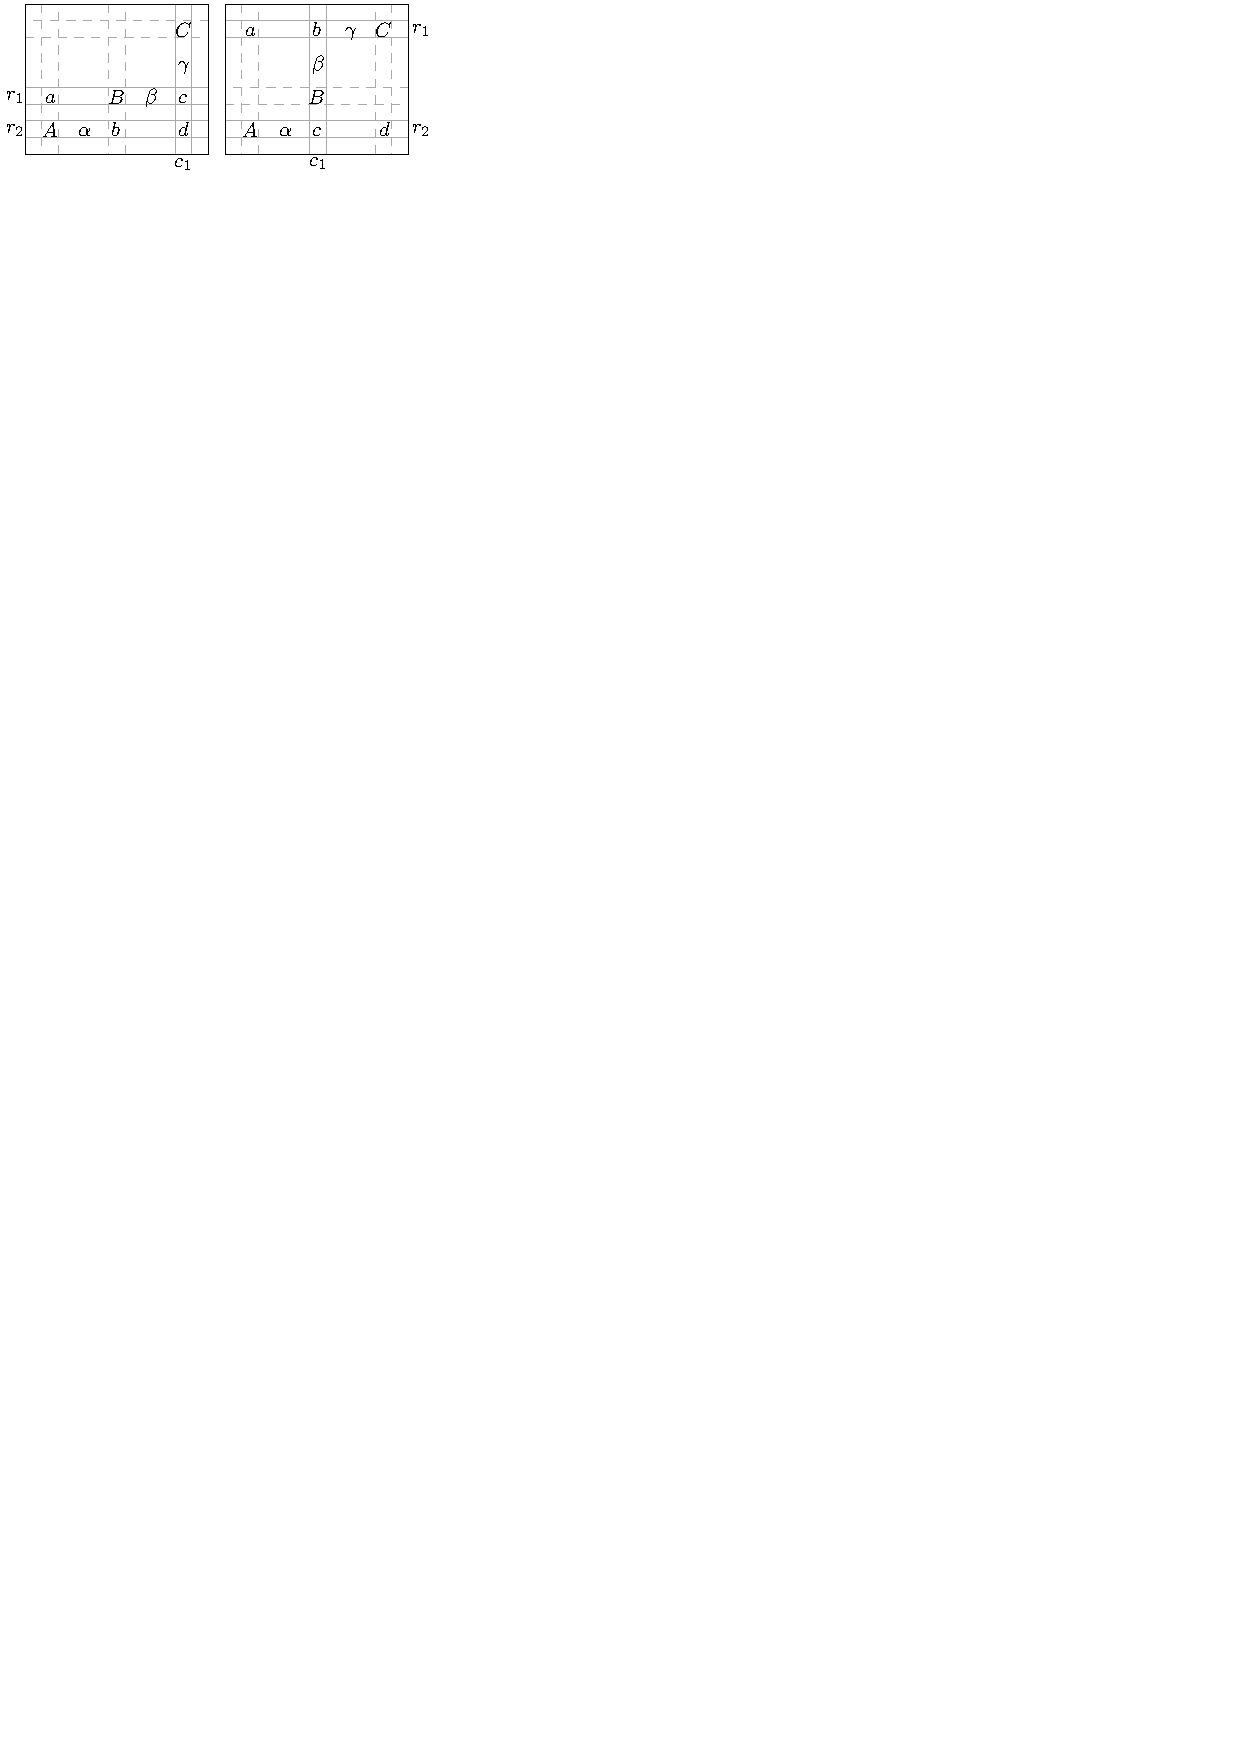
\includegraphics[width=110mm]{img/twoplusone.pdf}
	\caption{The structure of a pattern only having one-entries in two rows and one column that avoids all rotations of $P_1$.}
	\label{fig:twoplusone}
\end{figure}
\begin{enumerate}
\item $C$ lies in column~$c_1$
	\begin{enumerate}
		\item $a=0$
		\item $a=1\Rightarrow b=0,\ \alpha=0$
	\end{enumerate}
\item $B$ lies in column~$c_1$
	\begin{enumerate}
		\item $a=1,\ d=1\Rightarrow\alpha=0,\ \gamma=0$
		\item $a=1,\ d=0\Rightarrow\alpha=0$
		\item $a=0,\ d=1\Rightarrow\gamma=0$
		\item $a=0,\ d=0$. The pattern avoids $\smm{\bullet& \\ &\bullet}$.
	\end{enumerate}
\item $A$ lies in column~$c_1$. This is symmetric to the first situation.
\end{enumerate}
\begin{figure}[!ht]
	\centering
	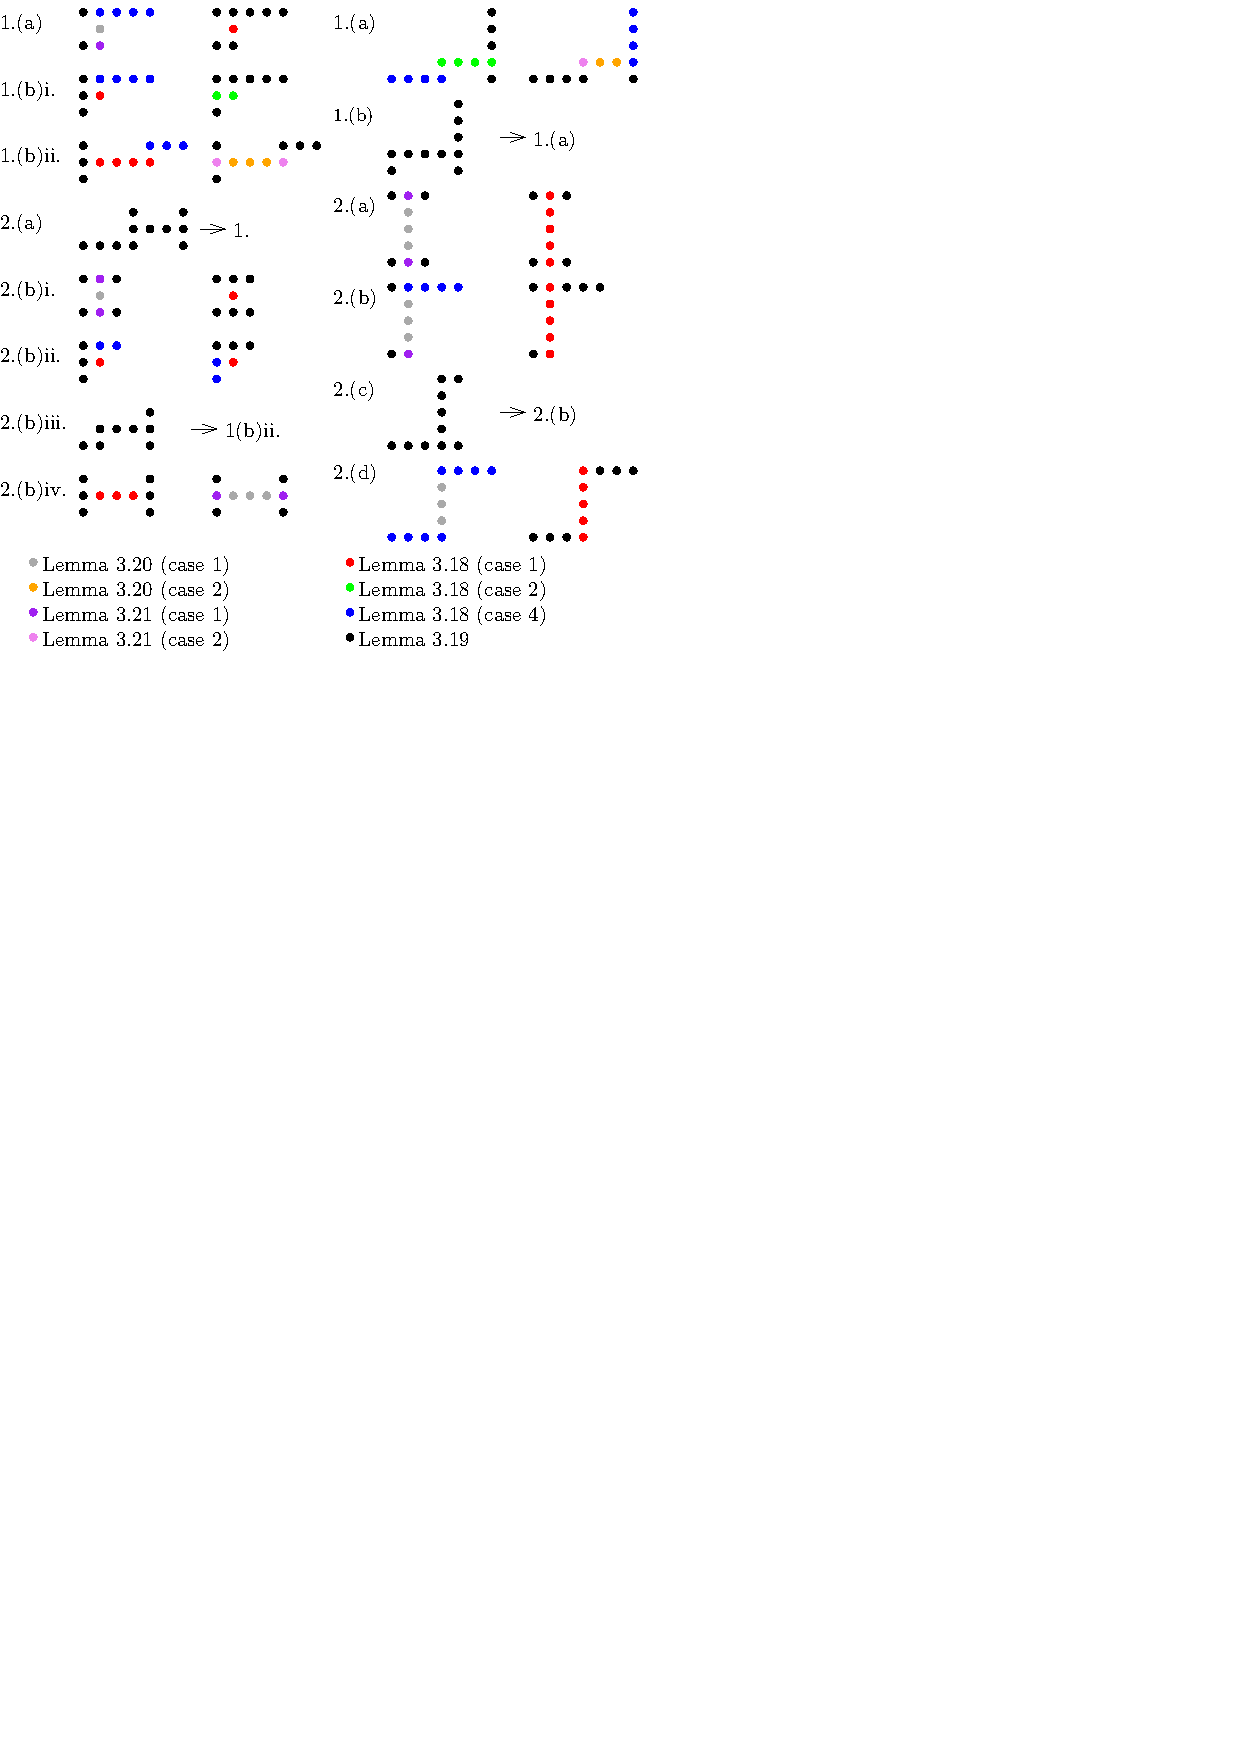
\includegraphics[width=120mm]{img/caseana.pdf}
	\caption{A figure showing which lemma can be used to prove that each one-entry of patterns discussed in the case analysis is bounded. The patterns from the left half of the picture only contain three non-empty rows and the patterns from the right half only contain two non-empty rows and one non-empty column. Each case either contains a picture showing that each one-entry is row-bounded and column-bounded, or an arrow describing that the case can be reduced to a different one.}
	\label{fig:pictproof1}
\end{figure}
The same analysis also proves that if a pattern~$P$ has two non-empty columns and one non-empty row then the pattern is bounding.
\end{proof}

Combining the lemmata we finally get the following result.

\begin{thm}
Let $P$ be a pattern avoiding all rotations of $P_1$, then $P$ is bounding. \qed
\end{thm}

A lot can be implied from this theorem. Here are two straightforward corollaries for which we do not know any other proof.

\begin{cor}
\label{cor:rowcol}
For every pattern $P$: $\Avm{P}$ is row-bounded $\Leftrightarrow\Avm{P}$ is column-bounded.
\end{cor}

\begin{cor}
For every bounding pattern $P$ and every $P'\im P$ it holds $P'$ is bounding.
\end{cor}

\section{Chain rules}
Now that we know exactly what patterns are bounding, it is time to speak about the complexity of classes more in general. We are still going to be concerned with classes of matrices avoiding patterns, but they will avoid a set of patterns rather than just one pattern.

First, we show that Corollary~\ref{cor:rowcol} does not hold in general. Next, we show that bounded classes are closed to intersection. At the end of the chapter, we prove the same is not true for unbounded classes of matrices and even more, an intersection of a few unbounded classes can be bounded hereditarily, which means that its every subset is bounded.

It is easy to see that Lemma~\ref{lemma:H}, Lemma~\ref{lemma:First}, Lemma~\ref{lemma:I}, Lemma~\ref{lemma:I2} and Lemma~\ref{lemma:walkpat} can be generalized to our settings. Their proofs without change show that for every set of patterns~$\class{P}$, if a pattern~$P\in\class{P}$ looks like a described pattern, then any one-entry of $P$ is (row-)bounded in $\Avm{\class{P}}$. Therefore, we use the lemmata without restating them.

We define classes of matrices to be bounded if they are both row-bounded and column-bounded. From what we proved so far, we see that for a pattern~$P$, the class~$\Avm{P}$ is row-bounded if and only of it is column-bounded. Once we consider classes avoiding sets of patterns, this does not have to be true.

\begin{lemma}
There exists a set of patters~$\class{P}$ such that the class~$\Avm{P}$ is row-bounded but column-unbounded.
\end{lemma}
\begin{proof}
Let $\class{P}=\left\lbrace P=\smm{ &\bullet& \\\bullet& & \\ &\bullet& \\ & &\bullet},I_4=\smm{\bullet& & & \\ &\bullet& & \\ & &\bullet& \\ & & &\bullet}\right\rbrace$. We can use a similar construction to what we did in Lemma~\ref{lemma:manyints}, to prove $\Avm{\class{P}}$ is column-unbounded. The only difference is that the ``blocks'' are of size $4\times2$ and the whole matrix is transposed.

To prove that the class~$\Avm{\class{P}}$ is row-bounded, we take an arbitrary matrix~$M\in\Avmax{\class{P}}$ and consider any row~$r$ of $M$. We need to prove that every one-entry of $I_4$ and $P$ is row-bounded.

From Lemma~\ref{lemma:walkpat}, we know that every one-entry of $I_4$ is row-bounded (and column-bounded) in $\Avm{\class{P}}$. From Lemma~\ref{lemma:First}, one-entries $P[2,1]$ and $P[4,3]$ are row-bounded in $\Avm{\class{P}}$. From the first case of Lemma~\ref{lemma:I}, the one-entry~$P[3,2]$ is row-bounded in $\Avm{\class{P}}$.

We prove that there are at most two zero-intervals usable for $P[1,2]$ in the row~$r$. For contradiction, let there be three zero-intervals~$z_1<z_2<z_3$. Consider a mapping of $P$ to $M$ created when a zero-entry of $z_3$ is changed to a one-entry used to map $P[1,2]$. Without loss of generality, the one-entry used to map $P[2,1]$ lies in columns of $z_3$ or just under the one-entry~$e$ bounding $z_3$ from left; otherwise, we could use $e$ to map $P[1,2]$ and find the pattern in $M$. Then, a one-entry between zero-intervals $z_1$ and $z_2$ together with the one-entries used to map $P[2,1],P[3,2]$ and $P[4,3]$ give us a mapping of $I_4$ and so a contradiction with $M\in \Avm{\class{P}}$.
\end{proof}

\begin{thm}
\label{thm:boundunion}
Let $\class{P}$ and $\class{Q}$ be classes of patterns. If both classes $\Avm{\class{P}}$ and $\Avm{\class{Q}}$ are bounded then $\Avm{\class{P}\cup\class{Q}}$ is bounded.
\end{thm}
\begin{proof}
Let $\class{R}=\class{P}\cup\class{Q}$. We show that $comp_{\class{R}}\leq comp_\mathcal{P}+comp_\mathcal{Q}=C$.

For contradiction, let a matrix $M\in\Avmax{\class{R}}$ have at least $C+1$ zero-intervals in a single row (or column). Without loss of generality, it means there is more than $comp_\class{P}$ zero-intervals usable for one-entries of the patterns from $\class{P}$. Let $M'\in\Avm{\class{P}}$ be a matrix created from $M$ by changing as many zero-entries to one-entries as possible. Clearly, it still contains more than $comp_\class{P}$ zero-intervals usable for one-entries of the patterns from $\class{P}$, which is a contradiction with the value of $comp_\class{P}$.
\end{proof}

Using induction, we can show that also a union of a finite number of bounded classes of finite sizes is bounded. Interestingly enough, unbounded classes are not closed the same way.

\begin{thm}
For every $1\leq i<j\leq4]$ is $\Avm{\{P_i,P_j\}}$ bounded.
\end{thm}
\begin{proof}
We only show that $\Avm{P_1,P_2}$ is bounded. To prove $\Avm{P_1,P_3}$ is bounded, we can use the same steps. All other pairs are then symmetric to these two.
\begin{itemize}
	\item $\Avm{P_1,P_2}$ is row-bounded:\\
	From Lemma~\ref{lemma:First}, we have that one-entries $P_1[2,1],P_1[3,3],P_2[2,3]$ and $P_3[3,1]$ are row-bounded. For $P_1[1,2]$ and $P_2[1,2]$, we prove there are at most two zero-intervals usable for each of them in each row of any matrix~$M\in\Avmax{P_1,P_2}$. For contradiction, let $z_1<z_2<z_3$ be three zero-intervals usable for $P_1[1,2]$ in a row~$r$ of $M$. The one-entries used to map $P_1[2,1]$ and $P_1[3,3]$ in a mapping created when a zero-entry of $z_1$ is changed to a one-entry used to map $P_1[1,2]$, together with a one-entry in between $z_2$ and $z_3$ give us a mapping of $P_2$ to $M$. Symmetrically, the same goes for $P_2[1,2]$.
	\item $\Avm{P_1,P_2}$ is column-bounded:\\
	The proof that all one-entries of $P_1$ and $P_2$ are column-bounded is the same.
\end{itemize}
\end{proof}

We prove even stronger result for the class~$\Avm{P_1,P_2,P_3,P_4}$ by using a well known fact from the theory of ordered sets. It is due to \cite{higman} and states the following:

\begin{fct}[Higman's lemma]
\label{fct:Higman}
Let $A$ be a finite alphabet and $A^*$ be a set of finite sequences over $A$ partially ordered by the subsequence relation. Then $A^*$ is well-quasi-ordered.
\end{fct}

In other words, whenever we have a potentially infinite $S\subseteq A^*$, there are sequences $a,b\in S$ such that $a$ is a subsequence of $b$. This also means that no such $S$ contains an infinite anti-chain.

\begin{thm}
The class~$\sigma=\Avm{P_1,P_2,P_3,P_4}$ is bounded. Moreover, its every subclass is bounded.
\end{thm}
\begin{proof}
While the previous two theorem already prove that $\sigma$ is bounded, we prove it by hand so that we can use the proofs to also show that every subclass of $\sigma$ is bounded.

From Theorem~\ref{thm:boundedints}, we know that elements of $\sigma$ fall into finitely many categories. For each of them, we need to prove that it is bounded and also that it does not contain an infinite anti-chain. Then we use Theorem~\ref{thm:boundunion} to obtain the result. Let us consider any $m\times n$ matrix $M\in\sigma$:
\begin{itemize}
	\item $M$ only contains up to three non-empty rows (columns):\\
		If $M$ is critical in $\sigma$ then it contains three rows made of one-entries and everything else is zero, so the number of one-intervals is bounded by three.\\
		
		To proof there is no infinite anti-chain, we use Fact~\ref{fct:Higman}. To describe $M$ we use words over alphabet~$A=\{a,b,c,d,e,f,g,h,i,j\}$. Let $r_1<r_2<r_3$ be the non-empty rows (if less then three are non-empty we choose extra values arbitrarily). We define $w_M\in A^*$ as follows. First, we use a letter~$g$ $r_1$ times, letter $h$ $r_2-r_1$ times, letter $i$ $r_3-r_2$ times and letter $j$ $m-r_3$ times to describe the number of rows of $M$ and position of non-empty rows. Then we describe columns from the first one to the last one as follows. For each 0 in $r_1$ we use a letter $a$ and for 1, we use letters $ab$. For each 0 in $r_2$ we use a letter $c$ and for 1, we use letters $cd$. For each 0 in $r_3$ we use a letter $e$ and for 1, we use letters $ef$.
		
		If we have $w_M,w_{M'}\in A^*$ such that $w_M$ is a subsequence of $w_{M'}$, then we want to show that $M$ is an interval minor of $M'$. Let $r_1,r_2,r_3$ and $r_1',r_2',r_3'$ be the non-empty rows of $M$ and $M'$ respectively. Since the number of leading letters $g$ is not bigger in $w_M$, $M$ does not have more empty rows before $r_1$ than $M'$ does before $r_1'$ and similarly for the other pairs of non-empty rows.

		Now consider there is $ab$ in $w_M$ and it corresponds to some $a\dots b$ in $w_{M'}$. Without loss of generality, the letter $a$ in $w_{M'}$ is the one exactly before $b$. Clearly, one-entries of $M$ can be mapped to one-entries in $M'$ and we only need to check that two one-entries of two different columns of $M$ are not mapped to two one-entries of the same column of $M'$. But this is not hard to see and we have $M\im M'$ (but it does not have to hold that $M\leq M'$).

		From Fact~\ref{fct:Higman}, we have that $A^*$ is well ordered, which means that matrices having at most three non-empty rows (columns) are well ordered and so they does not have an infitely long anti-chain.
	\item $M$ only contains at most two rows and one column (or vice versa):\\
		The number of one-intervals of any critical matrix $M$ is bounded by two.\\
		
		We use words over alphabet~$A=\{a,b,c,d,e,f,g\}$ and for non-empty rows~$r_1,r_2$ and column~$c_1$, we define $w_M$ as follows. We first encode each column in such a way that for each 0 in $r_1$ we use a letter~$a$ and for 1, we use letters~$ab$. For each 0 in $r_2$ we use a letter~$c$ and for 1, we use letters~$cd$. Right before and after the description of column $c_1$, we put a letter $g$. Next, we encode each row in such a way that for each 0 in $c_1$ we use a letter~$e$ and for each 1 letters~$ef$. Right before and after the descriptions of rows $r_1$ and $r_2$ we again place a letter~$g$.
		
		Because of the distinct letters for encoding rows and columns we can apply the same analysis as we did in the previous case and since entries at $M[r_1,c_1]$ and $M[r_2,c_1]$ are separated from the rest by a special letter~$g$ there is no way to find a one-entry if it is not there.
	\item $M$ avoids $\smm{ &\bullet\\\bullet& }$ (or $\smm{\bullet& \\ &\bullet}$):\\
		From Proposition~\ref{prop:walking} we know $M$ is a walking matrix and any such critical matrix only contains at most one one-intervals in each row and column.\\
		
		We use words over alphabet~$A=\{a,b,c,d\}$ and encode $M$ as follows. We choose an arbitrary walk of $M$ containing all one-entries and index its entries as $w_1\dots w_{m+n-1}$. Starting from $w_1$, we encode $w_i$ so that a letter~$a$ stands for 0 and letters~$ab$ for 1, if $w_{i+1}$ lies in the same row as $w_i$, and we use a letter~$c$ for 0 and letters~$cd$ for 1, if $w_{i+1}$ lies in the same column as $w_i$. We always use $a$ or $ab$ for the last entry.
\end{itemize}

In the construction of words corresponding to matrices, we only made sure that $w_M\subseteq w_{M'}\Rightarrow M\im M'$ and the other implication does not need to hold. A different construction may lead to equivalence, but that is not necessary for our result.

We use distinct alphabets to describe different categories and when given a potentially infinite class of matrices from $\sigma$, we know that inside each category there is at most finite number of minimal matrices such that all of the rest contain a smaller one as an interval minor. Using induction on Theorem~\ref{thm:boundunion}, we have that each category is bounded and by applying induction with Theorem~\ref{thm:boundunion} once again, we get that the union of the categories is also bounded.
\end{proof}

\begin{obs}
There exists a bounding pattern~$P$ having an unbounded subclass of $\Avm{P}$.
\end{obs}
\begin{proof}
Let $P=I_n$ (identity matrix) for $n>3$. From Lemma~\ref{lemma:walkpat}, we have that $P$ is bounding. On the other hand, $\Avm{I_n,P_1}$ is unbounded, because the construction used in the proof of Lemma~\ref{lemma:manyints} also works for this class.
\end{proof}

\section{Complexity of one-entries (probably to be delete)}
So far we have been working with the whole patterns and determining their complexity. To make the results even more general, we can analyze the complexity of each one-entry.

In spare time, I will have a look at this. 

\begin{lemma}
\label{lemma:cross}
Let $P\in\Pat$ be a pattern such that all its one-entries are either in rows $r_1,r_2$ ($r_1<r_2$) and $P[[r_2],\{c\}]$. Then $P[r_1,c]$ is row-bounded.
\end{lemma}
\begin{proof}
We prove there are at most $k^4$ zero-intervals usable for $P[r_1,c]$ in each row of any maximal matrix $M$ avoiding $P$. For contradiction, let there be more than $k^4$ of them ($zi_1,\dots,zi_{k^4}$) in some row and for each of them, consider the top most row $r'_j$ used to map $r_2$-th row of $P$ in a mapping created when a zero-entry of $zi_j$ is changed to a one-entry used to map $P[r_1,c]$. Then pairs $[zi_1,r'_1],[zi_2,r'_2],\dots,[zi_{k^4},r'_{k^4}]$ form a sequence of distinct pairs and thanks to the Pigeonhole principle, there is a subsequence of length at least $k^2$ such that the values of $r'_j$ are either non-increasing or non-decreasing. Without loss of generality, assume they are non-decreasing and let $zi'_1,\dots,zi'_{k^2}$ be their corresponding zero-intervals.

What if $P[r_2,c]=0$? TODO
\end{proof}

\begin{thm}
Let $P$ be a pattern. Any one-entry $P[r,c]$ is row-unbounded if (and only if) there is a trivially unbounded one-entry $P[r,c']$ and we cannot apply the fourth case of Lemma~\ref{lemma:H} nor Lemma~\ref{lemma:cross} to $P[r,c]$.
\end{thm}
\begin{proof}
Without loss of generality, let $P[r,c']$ be part of mapping of $P_1$, where $P_1[1,2]$ is mapped to it. Let $P_1[2,1]$ be mapped to $P[r_2,c_2]$ and $P_1[3,3]$ be mapped to $P[r_3,c_3]$. We go through all potential one-entries $P[r,c]$ and show that either we can use one of the lemmata mentioned in the statement or the one-entry is row-unbounded.
\begin{itemize}
	\item $c<c_2$: If there is no one-entry in $P[[r-1],[c-1]]$ nor $P[[r+1,k],[c-1]]$, then the fourth case of Lemma~\ref{lemma:H} can be used for $P[r,c]$. Otherwise, first consider there is a one-entry in $P[[r-1],[c-1]]$, then we can use the construction from Lemma~\ref{lemma:unbound2}. In the last case, assume there is a one-entry $P[r',c']$ in $P[[r+1,k],[c-1]]$, then if $r'!=r_2$, entries $P[r,c],P[r',c']$ and $P[r_2,c_2]$ form either $P_1$ or $P_2$ and $P[r,c]$ is trivially row-unbounded. If $r'=r_2$, then we use $P[r,c],P[r',c']$ and $P[r_3,c_3]$ to again find either $P_1$ or $P_2$ and $P[r,c]$ is trivially row-unbounded once again.
	\item $c=c_2$: If there is no one-entry in $P[[r-1],[c-1]]$ nor $P[[r+1,k],[c-1]]$, then the fourth case of Lemma~\ref{lemma:H} can be used for $P[r,c]$. Otherwise, first assume there is a one-entry in $P[[r-1],[c-1]]$, then we can use the construction from Lemma~\ref{lemma:unbound3}. In the last case, assume there is a one-entry $P[r',c']$ in $P[[r+1,k],[c-1]]$, then if $r'!=r_3$, entries $P[r,c],P[r',c']$ and $P[r_3,c_3]$ form either $P_1$ or $P_2$ and $P[r,c]$ is trivially row-unbounded. If $r'=r_3$, then what?
	
	Cannot just use lemma even if it was proved.
	
	TOOD
	\item $c_2<c<c_3$: In this case $P[r,c]$ is trivially unbounded as together with $P[r_2,c_2]$ and $P[r_3,c_3]$ it forms $P_1$.
	\item $c=c_3$: If there is no one-entry in $P[[r-1],[c+1,l]]$ nor $P[[r+1,k],[c+1,l]]$, then the fourth case of Lemma~\ref{lemma:H} can be used for $P[r,c]$. Otherwise, first consider there is a one-entry in $P[[r-1],[c+1,l]]$, then we can use the construction from Lemma~\ref{lemma:unbound3}. In the last case, assume there is a one-entry $P[r',c']$ in $P[[r+1,k],[c-1]]$, then if $r'!=r_2$, entries $P[r,c],P[r',c']$ and $P[r_2,c_2]$ form either $P_1$ or $P_2$ and $P[r,c]$ is trivially row-unbounded. If $r'=r_2$, then we use the construction from Lemma~\ref{lemma:unbound} to show $P[r,c]$ is row-unbounded once again.
	\item $c>c_3$: There are three cases to go through and we can handle them the same way as we did in case $c<c_2$.
\end{itemize}
\end{proof}